%------------------------------------------------------------------------------
% Copyright (c) !!COPYRIGHTYEAR!!, Xavier Leroy and Didier Remy.  
%
% All rights reserved. Distributed under a creative commons
% attribution-non-commercial-share alike 2.0 France license.
% http://creativecommons.org/licenses/by-nc-sa/2.0/fr/
%
% Translation by Richard Paradies
%------------------------------------------------------------------------------

\chapter{Files}
\label{sec/files}
\cutname{files.html}

The term \quotes{file} in Unix covers several types of objects:
%
\begin{itemize}
\item Standard files: Finite sets of bytes containing 
      text or binary information which we may call "ordinary" files.

\item Directories

\item Symbolic links

\item Specialized files (\emph{devices}), which give 
      specific types of access to computer peripherals

\item Named pipes

\item Sockets named in the Unix domain.
       
\end{itemize}
%
The representation of a file simultaneously contains the data 
contained in the file and information about the file (also
called meta-data) such as file type, access privileges, latest
access dates,{\etc}

\section{The File System}

As a first approximation, we may think of the file system as a tree. The
root is represented by \ml+'/'+ . The branches are labelled by the names (of  
the files), which are made up of strings of any characters excluding 
solely the characters  \ml+'\000'+ and \ml+'/'+,  but it is good practice
to avoid the use of non-printing characters as well as spaces.
The non-terminating nodes of the file system are
called \emph{directories}: These nodes always contain two branches \ml+.+
and {..} which respectively represents the directory itself and the directory's
parent. The other nodes are sometimes called "files",
as opposed to directories, but this is ambiguous, as we can also  
designate any node as a "file". To avoid all ambiguity 
we refer to them as \quotes{ordinary files}.

The nodes of the file system are represented by paths. These may refer to
the top of the file hierarchy or to a directory (usually the current
work directory) in which case we may refer to them as absolute
paths. A relative path is a string of file names separated by the the
character \ml+'/'+.  An absolute path is a relative path preceded by
the the character \ml+'/'+ (note the double use of of this character
both as a separator and as the name of the root node).

The \libmodule{Filename} library handles file paths in a portable
manner. Notably \libvalue{Filename}{concat} concatenates paths without
using the character \ml+'/'+, allowing the code to function equally
well on other architectures (for example the path separation character
under Windows is \texttt{'\char `\\'}).  Similarly, the \ml+Filename+
module provides the names \libvalue{Filename}{current\_dir\_name} and
\libvalue{Filename}{parent\_dir\_name} to represent the branches
\ml+.+ and \ml+..+.  The \libvalue{Filename}{basename} and
\libvalue{Filename}{dirname} functions extract the prefix \ml+d+ and
the suffix \ml+b+ from a file path \ml+p+ such that the file path
\ml+p+ and \ml+d/b+ refer to the same file, where \ml+d+ refers to the
directory in which the file is found and \ml+b+ the name of the file
within the directory.

The functions defined in \ml+Filename+ operate only on files,
independently of their position within the file hierarchy.
In fact, the file hierarchy is not a tree.  In particular, the
directory conventions \ml+.+ and \ml+..+ allow the directory to refer
to itself (auto-referencing) and allow remounting within the file
hierarchy, thus allowing the creation of paths in a directory leading
to itself.  In addition, non-directory files can have many
ancestors. In this case, one says that they have many \quotes{hard
  links}. Finally, there are also \quotes{symbolic links} which lend
themselves to a double interpretation.  A symbolic link is a
non-directory file which contains a path.  Additionally, a symbolic
link can be interpreted as an ordinary file and we can simply read
what it contains, a link.  It is also possible to follow the symbolic
link in a transparent manner and not see anything but the target file.  
The latter is the only possible interpretation when the link appears in
the middle of a file path: if \ml+s+ is a symbolic link whose value is
the path \ml+l+, then the path \ml+p/s/q+ represents the file \ml+l/q+
if \ml+l+ is an absolute link or the file \ml+p/l/q+ if \ml+l+ is a
relative link.

\begin{myfigure}
\begin{myimage}[width="100\%"]
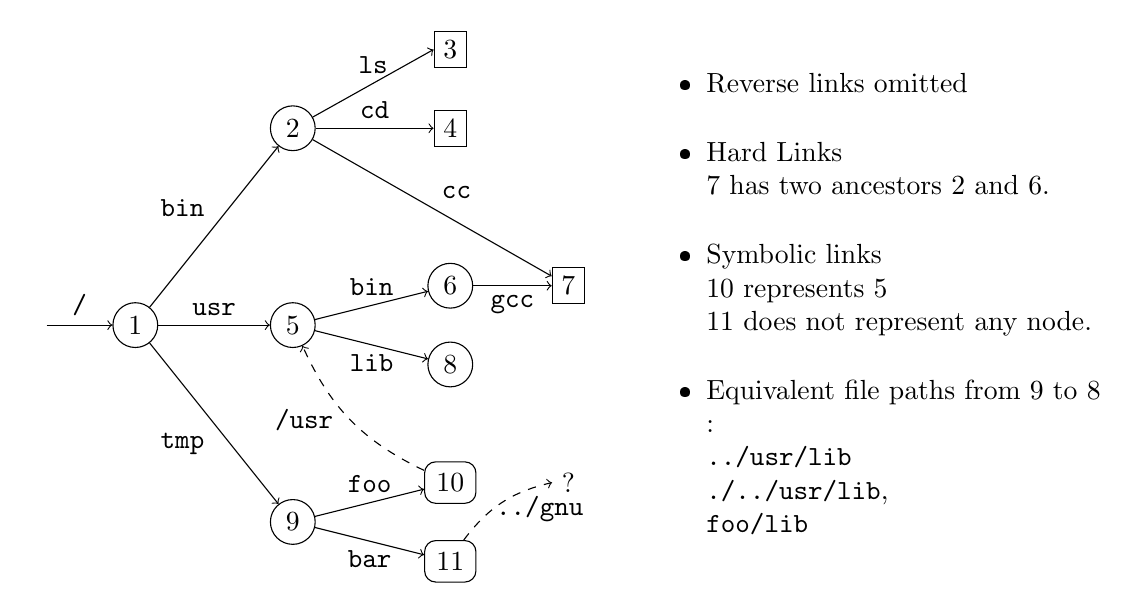
\begin{tikzpicture}
[dir/.style={draw, circle, inner sep=1mm},
 slink/.style={draw,rectangle,inner sep=1.5mm, rounded corners},
 file/.style={draw,rectangle},
 tpath/.style={font={\ttfamily},midway}]
\node (start) at (-1.25,0) {};
\node (n1) at (0,0) [dir] {1};

\node (n2) at (2,2.5) [dir] {2};
\node (n5) at (2,0) [dir] {5};
\node (n9) at (2,-2.5) [dir] {9};

\node (n3) at (4,3.5) [file] {3};
\node (n4) at (4,2.5) [file] {4};
\node (n6) at (4,0.5) [dir] {6};
\node (n8) at (4,-0.5) [dir] {8};
\node (n10) at (4, -2) [slink] {10};
\node (n11) at (4, -3) [slink] {11};

\node (n7) at (5.5, 0.5) [file] {7};
\node (nqmark) at (5.5, -2) {?};

\draw[->] (start) to node [tpath,above] {/} (n1);

\draw[->] (n1) to node [tpath,above left] {bin} (n2);
\draw[->] (n1) to node [tpath,above] {usr} (n5);
\draw[->] (n1) to node [tpath,below left] {tmp} (n9);

\draw[->] (n2) to node [tpath,above] {ls} (n3.west);
\draw[->] (n2) to node [tpath,above] {cd} (n4);
\draw[->] (n2) to node [tpath,above right] {cc} (n7);

\draw[->] (n5) to node [tpath,above] {bin} (n6);
\draw[->] (n5) to node [tpath,below] {lib} (n8);

\draw[->] (n9) to node [tpath,above] {foo} (n10);
\draw[->] (n9) to node [tpath,below] {bar} (n11);

\draw[->] (n6) to node [tpath,below] {gcc} (n7);

\draw[->,dashed] (n10) to [bend left=20] node [tpath,left=1mm] {/usr} (n5);
\draw[->,dashed] (n11) to [bend left=20] node [tpath,below right=-2mm] {../gnu} (nqmark.west);
\node[right=0.75cm, text width=6cm] at (n7)
{
  \begin{itemize}
    \item Reverse links omitted \vspace{5pt}
    \item Hard Links \\ 
      7 has two ancestors 2 and 6.\vspace{5pt}
    \item Symbolic links \\ 
      10 represents 5 \\ 
      11 does not represent any node. \vspace{5pt}
    \item Equivalent file paths from  9 to 8 : \\
      \texttt{../usr/lib} \\
      \texttt{./../usr/lib}, {\etc} \\
      \texttt{foo/lib}
  \end{itemize}
};
\end{tikzpicture}
\end{myimage}
\caption{An example of a file hierarchy}
\label{fig/hierarchy}
\end{myfigure}

Figure~\ref{fig/hierarchy} gives an example of a file hierarchy.  The
symbolic link \ml+11+ referred to by the file path \ml+/tmp/bar+,
where the value is the relative path \ml+./gnu+, does not refer to any
existing file in the hierarchy (in this instant).

In general, a recursive traversal of the hierarchy will be complete
if the following two rules are followed:
%
\begin{itemize}
\item the directories \ml+currentdir+ and \ml+parentdir+ are ignored.
\item symbolic links are not followed. 
\end{itemize}
%
If a symbolic link is followed, one is brought back to a
traversal of the graph and care is required to keep track of nodes we
have already visited and nodes that we are currently visiting.

Each process has a current working directory. It is possible to check what
this is using the function \indexlibvalue{Unix}{getcwd} and it can
be changed by passing a desired target directory to
\indexlibvalue{Unix}{chdir}.  It is also possible to constrict the view
of the file hierarchy using \indexlibvalue{Unix}{chroot}\ml+ p+ which
makes the node \ml+p+, which should be a directory, the root of the 
of a restricted view of the hierarchy.  Absolute file paths
are then interpreted in accordance with the new root (trying to access
the path \ml+..+ from the root of the chroot is not possible).

\section{File names, file descriptors}

There are two methods of accessing a file.  The first is by its
\emph{name}, or \emph{file access path} in the file system hierarchy.
A file can have many different names as a result of hard links.
The names are represented by strings of characters (type \ml+string+). 
Here are some examples of system calls that operate on the file name level. 

\syscall{unlink}, \syscall{link}, \syscall{symlink} and \syscall{rename} 
%
\begin{listingcodefile}{tmpunix.mli}
val $\indexlibvalue{Unix}{unlink}$ : string -> unit
val $\indexlibvalue{Unix}{link}$ : string -> string -> unit
val $\indexlibvalue{Unix}{symlink}$ : string -> string -> unit
val $\indexlibvalue{Unix}{rename}$ : string -> string -> unit
\end{listingcodefile}
%
The call \ml+unlink f+ erases the file \ml+f+ given in the argument (like
the command \ml+rm -f f+),
%
\ml+link f1 f2+ create a hard link named \ml+f2+ on the file named  
\ml+f1+ (like the command \ml+ln f1 f2+), 
% 
\ml+symlink f1 f2+ create a symbolic link named \ml+f2+ to the file  
named  \ml+f1+ (like the command \ml+ln -s f1 f2+) and
%
\ml+rename f1 f2+ renames the file with name \ml+f1+ to \ml+f2+  (
like the command \ml+mv f1 f2+).

The other method of accessing a file is through a file descriptor.  A
descriptor contains a pointer to a file in addition to other
information like the current reading/writing position in the file,
the permissions on the file (read-permission ? write-permission ?)
and the wrappers which control the behavior of the read and write
processes (writes appending or overwriting blocking reads or
non-blocking).  The descriptors are represented by values of abstract
type \libtype{Unix}{file\_descr}.

File access through a descriptor is in large part independent
of access via the file name.  In particular, when a 
descriptor for a file is obtained, the file may be destroyed or renamed
but the descriptor will always point to the original file.

When a program is launched, three descriptors are allocated and 
tied to variables \ml+stdin+, \ml+stdout+ and \ml+stderr+ of the
\ml+Unix+ module:
\begin{codefile}{tmpunix.mli}
type file_descr
\end{codefile}
\begin{listingcodefile}{tmpunix.mli}
val $\indexlibvalue{Unix}{stdin}$ : file_descr
val $\indexlibvalue{Unix}{stdout}$ : file_descr
val $\indexlibvalue{Unix}{stderr}$ : file_descr
\end{listingcodefile}

They correspond respectively to the standard input of the process, the
standard output of the process and the standard error of the process.

When a program is launched interactively on the command line and
without any redirections, the three descriptors refer to the terminal.
But if, for example, the input has been redirected by the notation 
\ml+cmd < f+, then the descriptor \ml+stdin+ refers to the file with
file name \ml+f+ during the execution of the command \ml+cmd+.

Similarly, \ml +cmd > f+ and \ml+cmd 2> f+ respectively act in such a
way that the descriptors \ml+stdout+ and \ml+stderr+ refer to the file
\ml+f+ during the execution of the command \ml+cmd+.


\section{Meta-attributes, types and permissions}

The system calls  \syscall{stat}, \syscall{lstat} and \syscall{fstat}
return the meta-attributes of a file. This is to say 
information about the node itself rather than its content.

Among other things, this information contains the identity of the file, the  
type of file, the access rights, the time and date of last access and other
auxiliary information.
%
\begin{codefile}{tmpunix.mli}
type stats
\end{codefile}
%
\begin{listingcodefile}{tmpunix.mli}
val $\libvalue{Unix}{stat}$  : string -> stats
val $\libvalue{Unix}{lstat}$ : string -> stats
val $\libvalue{Unix}{fstat}$ : file_descr -> stats
\end{listingcodefile}
%
The system calls \ml+stat+ and \ml+lstat+ take a file name as an 
argument.  The call \ml+fstat+ takes as an argument a previously opened descriptor 
and gives information about the specified file. The
difference between  \ml+stat+ and \ml+lstat+ can be seen in symbolic links
: \ml+lstat+  returns information on the symbolic link itself
, while \ml+stat+ returns information
about the file that the link refers to. 
%
The result of these three calls is a \emph{record} of type
\ml+stats+ described in the table~\ref
{fig/stats}.

\begin{mytable}
\begin{tabular}{lp{9cm}}
\ml+st_dev : int+ 
& The device number of the device where the file is located. \\
\ml+st_ino : int+ 
& The file's inode number in its partition. 
The tuple \ml+(st_dev, st_ino)+ uniquely identifies the file
within the file system. \\
\ml+st_kind : file_kind+ & 
The file type. The file type \ml+file_kind+ is an enumerated type
whose constructors are~:  
\begin{center}
\begin{tabular}{ll}
\ml+S_REG+ & regular file \\
\ml+S_DIR+ & directory \\
\ml+S_CHR+ & character device  \\
\ml+S_BLK+ & block device  \\
\ml+S_LNK+ & symbolic link \\
\ml+S_FIFO+ & named pipe \\
\ml+S_SOCK+ & socket 
\end{tabular}
\end{center}
\\
\ml+st_perm : int+ & Access rights for the file \\
\ml+st_nlink : int+ 
& For a directory: the number of entries in the directory. For others:
the number of hard links for this file. \\
\ml+st_uid : int+ & The user id of the file's owner. \\
\ml+st_gid : int+ & The group id of the file. \\
\ml+st_rdev : int+ 
& The associated major device number (through special files). \\
\ml+st_size : int+ & The size of the file, in bytes. \\
\ml+st_atime : int+ & The date the file's contents were last accessed..
(In seconds after January 1, 1970 midnight). \\
\ml+st_mtime : int+ & The date the file was last modified. (Idem.) \\
\ml+st_ctime : int+ & The date of the last change in the state of the file:
Either a  successful write to the file, or a successful change in access rights 
or change  of the owner, of the group, or the number of links.
\end{tabular}
\caption{Fields of the \ml+stats+ structure}
\label{fig/stats}
\end{mytable}


\subsection*{Identification}
A file is uniquely identified by a pair made up of its
device number (typically the disk partition where it is located)
\ml+st_dev+ and its inode number \ml+st_ino+. 

\subsection*{Owners}

A file has one user owner \ml+st_uid+ and one group owner
\ml+st_gid+.  All the users and user groups 
on the machine are usually described in the  
 \ml+/etc/passwd+ and \ml+/etc/groups+ files.  One can examine them by name  
in a portable manner through the help of the commands \syscall{getpwnam} and 
\syscall{getgrnam} or numerically through the help of the commands 
\syscall{getpwuid} and \syscall{getgrgid}.
%
\begin{codefile}{tmpunix.mli}
type passwd_entry = Unix.passwd_entry
type group_entry = Unix.group_entry
\end{codefile}
%
\begin{listingcodefile}{tmpunix.mli}
val $\libvalue{Unix}{getpwnam}$ : string -> passwd_entry
val $\libvalue{Unix}{getgrnam}$ : string -> group_entry
val $\libvalue{Unix}{getpwuid}$ : int -> passwd_entry
val $\libvalue{Unix}{getgrgid}$ : int -> group_entry
\end{listingcodefile}

The name of the user of a process which is running and all the groups
to whom it belongs can be retrieved with the commands
\syscall{getlogin} and \syscall{getgroups}.
%
\begin{listingcodefile}{tmpunix.mli}
val $\libvalue{Unix}{getlogin}$ : unit -> string
val $\libvalue{Unix}{getgroups}$ : unit -> int array
\end{listingcodefile}

The call  \syscall{chown} changes the owner (second argument) and 
the group (third argument) of a file (first
argument).  Only the super user can make these changes.
If the program has an open files descriptor on a file, one should
use \syscall{fchown} through the descriptor instead of \syscall{chown}
on the file name.
%
\begin{listingcodefile}{tmpunix.mli}
val $\libvalue{Unix}{chown}$ : string -> int -> int -> unit
val $\libvalue{Unix}{fchown}$ : file_descr -> int -> int -> unit
\end{listingcodefile}

%% Le changement de groupe peut se faire sans privil�ge lorsque le
%% programme � un \ml+uid+ (effectif) �gal � celui du fichier et un
%% \ml+gid+ (effectif) �gal au group d�sir� ou � un de ses groupes
%% suppl�mentaire


\subsection*{Access rights}

Access rights are encoded as bits in an integer and the type 
\libtype{Unix}{file\_perm} is just a synonym for the type
\ml+int+. Access rights specify read, write and execute rights 
for the user, the group and other, and other
special bits.  Access right are thus represented by a vector of bits:
%
\ifhtmlelse{%
\begin{center}
\begin{tabular}{ccc|ccc|ccc|ccc}
\multicolumn{3}{c}{\texttt{S}pecial}
&\multicolumn{3}{c}{\texttt{U}ser}
&\multicolumn{3}{c}{\texttt{G}roup}
&\multicolumn{3}{c}{\texttt{O}ther} \\
\hline
--&--&--&--&--&--&--&--&--&--&--&--\\
\hline
\multicolumn{12}{c}{\ml+OoSUGO+}
\end{tabular}
\end{center}
}
{%
\begin{displaymath}
\underbrace
{\overbrace{---}^{\texttt Special}
 \overbrace{---}^{\texttt User}
 \overbrace{---}^{\texttt Group}
 \overbrace{---}^{\texttt Other}}_{\texttt{0oSUGO}}
\end{displaymath}
}
%
where the order of bits in each of the user, group and other fields 
the read (\ml+r+), write  (\ml+w+) and execution rights of the file are indicated.
(\ml+x+). The permissions on a file result from the union of these respective permissions:
\begin{center}
\begin{tabular}{lcl}
Bit (octal) & Notation \ml+ls -l+ & Right \\
\hline
\ml+0o100+ & \ml+--x------+ & executable by the owner \\
\ml+0o200+ & \ml+-w-------+ & writable by the owner \\
\ml+0o400+ & \ml+r--------+ & readable by the owner \\
\hline
\ml+0o10+  & \ml+-----x---+ &
        executable by members of the owner's group. \\
\ml+0o20+  & \ml+----w----+ &
        writable by members of the owner's group. \\
\ml+0o40+  & \ml+---r----+ &
        readable by members of the owner's group. \\
\hline
\ml+0o1+   & \ml+--------x+ & executable by other users\\
\ml+0o2+   & \ml+-------w-+ & writable by other users \\
\ml+0o4+   & \ml+------r--+ & readable by other users \\
\hline
\ml+0o1000+ & \ml+--------t+ & the bit \ml+t+ on the group (sticky bit)\\
\ml+0o2000+ & \ml+-----s---+ & the bit \ml+s+ on the group (\ml+set-gid+)\\
\ml+0o4000+ & \ml+--s------+ & the bit \ml+s+ on the user (\ml+set-uid+)\\
\hline
\end{tabular}
\end{center}

The meaning of read and write permissions is clearer than 
that of the execution rights. Execution rights on a directory
mean the user's right to use the directory as a working directory (to
\ml+chdir+ into the directory ). Read permissions on a directory
are sufficient to list the directory's contents but not to read
its files or sub-directories (but it is sufficient to read their names).

The special bits do not have meaning unless the \ml+x+ bit is present. 
(when they are present without the bit \ml+x+, they do not give 
additional rights.  That is why their representation is superimposed
on that of bit \ml+x+ and the letters \ml+S+ and \ml+T+ are used instead of 
\ml+s+ and \ml+t+  while the bit \ml+x+ is not 
simultaneously present. The bit \ml+t+ allows sub-directories
to inherit the permissions of the parent directory. The bit \ml+s+
on a directory, allows the use of the owner's \ml+uid+ and \ml+gid+ 
rather than the user's in the creation 
of directories. The bit \ml+s+ on an executable file permits  
changing the user's or group's \emph{effective identity} at launch, 
(\syscall{setuid}) or of the group  (\syscall{setgid}).
%
\begin{listingcodefile}{tmpunix.mli}
val $\libvalue{Unix}{setuid}$ : int -> unit
val $\libvalue{Unix}{setgid}$ : int -> unit
\end{listingcodefile}
%
The process also preserves its original identities except when 
it has super user privileges, in which case, \ml+setuid+ and
\ml+setgid+ change its effective and original user and group identities 
at the same time. The original identity is preserved to allow 
the process to subsequently recover it as its effective identity without the need   
for further privileges. The system calls \syscall{getuid} and 
\syscall{getgid} return the original identities and 
\syscall{geteuid} and \syscall{getegid} return the effective identities.
%
\begin{listingcodefile}{tmpunix.mli}
val $\libvalue{Unix}{getuid}$ : unit -> int
val $\libvalue{Unix}{geteuid}$ : unit -> int
val $\libvalue{Unix}{getgid}$ : unit -> int
val $\libvalue{Unix}{getegid}$ : unit -> int
\end{listingcodefile}

A process also has a file creation mask made up in the same fashion. 
As its names indicates, the mask specifies prohibitions (masked permissions):
During file creation all the bits that have 1 in the creation mask  
are set to 0 in the permissions of the created file. The mask may be  
looked up and changed by the system call system \syscall{umask}~:
%
\begin{listingcodefile}{tmpunix.mli}
val $\libvalue{Unix}{umask}$ : int -> int
\end{listingcodefile}
%
Like the numerous system calls which modify a system variable,
the modifying function returns the old value of the variable.
By simply looking up the value, it can thus be modified twice
once with an arbitrary value, then the old value can be  
put back in place. For example, by doing  
%
\begin{codefile}{tmpfich.ml}
open Unix;;
let _ = 
\end{codefile}
%
\begin{listingcodefile}{tmpfich.ml}
let m = umask 0 in ignore (umask m); m
\end{listingcodefile}

File access permissions may be modified by the call
\syscall{chmod} and \syscall{fchmod}~:
%
\begin{codefile}{tmpunix.mli}
type file_perm
\end{codefile}
%
\begin{listingcodefile}{tmpunix.mli}
val $\libvalue{Unix}{chmod}$ : string -> file_perm -> unit
val $\libvalue{Unix}{fchmod}$ : file_descr -> file_perm -> unit
\end{listingcodefile}

File access rights may also be tested \quotes{dynamically} 
with the system call \syscall{access}
%
\begin{listingcodefile}{tmpunix.mli}
type $\libtype{Unix}{access\_permission}$ = R_OK | W_OK | X_OK | F_OK
val $\libvalue{Unix}{access}$ : string -> access_permission list -> unit 
\end{listingcodefile}
%
where required access rights to the file are given by the type
\ml+access_permission+ in which the meaning is obvious save for \ml+F_OK+
which only signifies that the file exists (possibly without
the process having the corresponding rights).

Note that \ml+access+ may return information more restrictive  
than that calculated from the static information used by 
\ml+lstat+ because a file hierarchy may be mounted 
with more restricted rights, for example read only. In this case
\ml+access+ will deny write permission although the information 
contained in the meta-attributes relative to the file
would allow it.  This is why we speak of \quotes{dynamic} information 
(that which the process can actually do) in  
contrast to \quotes{static} (that which the file system specifies).

\section{Operations on directories}

Only the kernel can write in directories (when files are
created). Thus opening a directory in write mode is prohibited. In
certain versions of unix a directory may be opened in read
only mode and read with \indexvalue{read}, but other versions
prohibit it. While this is possible, it is preferable 
not to do so because the format of directory entries vary
depending on the unix version and is often complex. The following functions
allow reading a directory sequentially in a manner that is
portable:
%
\begin{codefile}{tmpunix.mli}
type dir_handle = Unix.dir_handle
\end{codefile}
%
\begin{listingcodefile}{tmpunix.mli}
val $\libvalue{Unix}{opendir}$   : string -> dir_handle
val $\libvalue{Unix}{readdir}$   : dir_handle -> string
val $\libvalue{Unix}{rewinddir}$ : dir_handle -> unit
val $\libvalue{Unix}{closedir}$  : dir_handle -> unit
\end{listingcodefile}
%
The system call \syscall{opendir} returns a read descriptor
on a directory.  \syscall{readdir} reads the next entry of a
directory (or triggers the exception \ml+End_of_file+ if the end
of the directory is reach). The returned string consists of the name of the file
relative to the read directory. \syscall{rewinddir} repositions the 
descriptor at the beginning of the directory and \syscall{closedir} closes the
directory descriptor. 

To create a directory or remove an empty directory, we have
\syscall{mkdir} and \syscall{rmdir}~:
%
\begin{listingcodefile}{tmpunix.mli}
val $\libvalue{Unix}{mkdir}$ : string -> file_perm -> unit
val $\libvalue{Unix}{rmdir}$ : string -> unit
\end{listingcodefile}
%
The second argument of  \ml+mkdir+ encodes the access rights given to the
new directory.  Note that we can only remove a directory 
that is already empty. To remove a directory and its contents, it is thus
necessary to first recursively empty the contents of the directory then
remove the directory.

For example, we can write a function of general interest in the  
module \ml+Misc+  which iterates over the entries in a directory.
%
\begin{codefile}{misc.mli}
(*** Directory iterator *)
val iter_dir : (string -> 'a) -> string -> unit
(** [iter_dir f d] opens path [d] as a directory and iterates the 
function [f] over all its entries *)
\end{codefile}
%
\begin{codefile}{misc.ml}
open Sys;;
open Unix;;
\end{codefile}
%
\begin{listingcodefile}{misc.ml}
let iter_dir f dirname =
  let d = opendir dirname in
  try while true do f (readdir d) done
  with End_of_file -> closedir d
\end{listingcodefile}

\section {Complete example : search in a file hierarchy}
\label{ex/find}

The unix command \ml+find+ allows the recursive search of files 
in the hierarchy according to certain criteria (file  name, type and
permissions) etc. Here we propose to develop  part of
a library function \ml+Findlib.find+ which will allow us to 
make such searches and a command \ml+find+ providing a restricted
version of the unix command \ml+find+ does not implement any but the options
\ml+-follow+ and \ml+-maxdepth+.

We specify the following interface for the library \ml+Findlib+:
%
\begin{listingcodefile}{findlib.mli}
val find : 
  (Unix.error * string * string -> unit) -> 
  (string -> Unix.stats -> bool) -> bool -> int -> string list -> 
  unit
\end{listingcodefile}
%
The function call
\begin{lstlisting}
find handler action follow depth roots
\end{lstlisting}
traverses the file hierarchy starting from the indicated roots in
the list \ml+roots+ (absolute or relative to the current directory
when the call is made) up to a maximum depth \ml+depth+, following
symbolic links if the flag \ml+follow+ is set.  The paths 
found under the root \ml+r+ include \ml+r+ as a prefix.
Each found path \ml+p+ is passed to a function \ml+action+. Actually,
\ml+action+ also receives the data \ml+Unix.stat p+
if the flag \ml+follow+ is set or \ml+Unix.lstat p+ if not. The
function \ml+action+ returns a boolean, \ml+true+ in the case
where it was able to follow the search to the required depth
or \ml+false+ if it was interrupted.


The function \ml+handler+ serves to handle run-time errors,
necessarily of type \ml+Unix_errors+:  Exception arguments
are then sent to the function \ml+handler+ and execution
continues.  In case of an interrupt, the exception is passed up to 
the calling function. When an exception is raised by the functions
\ml+action+ or \ml+handler+, it stops the execution abruptly  
and is immediately passed up to the caller.

     
%% De plus on arr�te la visite r�cursive d'un r�pertoire que l'on est en train
%% de visiter (ce qui ne peut arriver que lorsqu'on suit les liens symboliques)

To pass an exception \ml+Unix_error+ without it being trapped
like a runtime error, we wrap it in another exception.
\begin{listingcodefile}[style=numbers]{findlib.ml}
open Unix;;

exception Hidden of exn
let hide_exn f x = try f x with exn -> raise (Hidden exn);;
let reveal_exn f x = try f x with Hidden exn -> raise exn;;

let find on_error on_path follow depth roots =
  let rec find_rec depth visiting filename =
    try
      let infos = (if follow then stat else lstat) filename in
      let continue = hide_exn (on_path filename) infos in
      let id = infos.st_dev, infos.st_ino in $\label{prog:did}$
      if infos.st_kind = S_DIR && depth > 0 && continue &&
        (not follow || not (List.mem id visiting))
      then
        let process_child child = 
          if (child <> Filename.current_dir_name &&
              child <> Filename.parent_dir_name) then 
            let child_name = Filename.concat filename child in
            let visiting = 
              if follow then id :: visiting else visiting in $\label{prog:follow}$
            find_rec (depth-1) visiting child_name in
        Misc.iter_dir process_child filename 
    with Unix_error (e, b, c) -> hide_exn on_error (e, b, c) in
  reveal_exn (List.iter (find_rec depth [])) roots;;
\end{listingcodefile}

Directories are identified by the pair \ml+id+
(line~\ref{prog:did}) which consists of their device number and
their inode. The list \ml+visiting+ contains all the directories
which have not yet been visited. Actually this information
is not useful unless symbolic links are followed
(line~\ref{prog:follow}).

We can now easily infer the function \ml+find+.
\begin{listingcodefile}{find.ml}
let find () =
  let follow = ref false in
  let maxdepth = ref max_int in
  let roots = ref [] in
  let usage_string  =
    ("Usage: " ^ Sys.argv.(0) ^ " [files...] [options...]") in
  let opt_list =  [ 
    "-maxdepth", Arg.Int ((:=) maxdepth), "max depth search";
    "-follow", Arg.Set follow, "follow symbolic links";
  ] in
  Arg.parse opt_list (fun f -> roots := f :: !roots) usage_string;
  let action p infos = print_endline p; true in
  let errors = ref false in
  let on_error (e, b, c) =
    errors := true; prerr_endline (c ^ ": " ^ Unix.error_message e) in
  Findlib.find on_error action !follow !maxdepth 
    (if !roots = [] then [ Filename.current_dir_name ] 
     else List.rev !roots);
  if !errors then exit 1;; 

Unix.handle_unix_error find ();;
\end{listingcodefile}
%

The essential part of the code consists of the analysis of the command 
line, for which we use the library module
\libmodule{Arg}.
%
\begin{codefile}{find.test}
cd ../../lib/arch
./find.byte -follow -maxdepth 10 A B > find.out
find A B -follow -maxdepth 10 | diff - find.out
rm find.out
\end{codefile}

Although the \ml+find+ function above is sufficiently 
restricted, the library function \ml+FindLib.find+ is
far more general, as the following exercise demonstrates.
\begin{exercise}

Use the library function \ml+FindLib+ to write a program
\ml+find_but_CVS+ equivalent to the Unix command 
\begin{lstlisting}
find . -type d -name CVS -prune -o -print
\end{lstlisting}
which recursively prints the files starting from the current directory
but without seeing (neither printing nor visiting) the directories by name
\ml+CVS+.
\end{exercise}
\begin{answer}
\begin{codefile}{find_but_CVS.ml}
open Unix;;
open Misc;;
\end{codefile}
%
\begin{listingcodefile}{find_but_CVS.ml}
let main () = 
  let action p infos = 
    let b = not (infos.st_kind = S_DIR || Filename.basename p = "CVS") in
    if b then print_endline p; b in
  let errors = ref false in
  let error (e,c,b) = 
    errors:= true; prerr_endline (b ^ ": " ^ error_message e) in
  Findlib.find error action false max_int [ "." ];;
handle_unix_error main()
\end{listingcodefile}
\end{answer}

\begin{exercise}
The function \ml+getcwd+ is not a system call but is defined in the 
library.  Give a \quotes{simple} implementation of
\ml+getcwd+. Describe the algorithmic principle. After which write
the algorithm (You should avoid repeating the same system call).
\end{exercise}
\begin{answer}
Here are some clues: We start back up from our current position  
towards the root away from the path which we are looking for.
The root is identified as the unique directory node
where the parent and the current directory are identical (the paths \ml+parentdir+ and 
\ml+currentdir+ are equal when they are taken relative to the  
root).  To find the name which represents a directory  \ml+r+ and then 
its parent directory, it is necessary to traverse all the parent names  
and identify the files they represent \ml+r+.
\end{answer}


\section{Opening a file}

The \ml+openfile+ function allows us to obtain a descriptor on
a file with a specific name (the corresponding system call
is \syscall{open}, however \ml+open+ is a keyword in {\ocaml}).
%
\begin{codefile}{tmpunix.mli}
type open_flag = Unix.open_flag;;
\end{codefile}
%
\begin{listingcodefile}{tmpunix.mli}
val $\libvalue{Unix}{openfile}$ : 
 string -> open_flag list -> file_perm -> file_descr
\end{listingcodefile}
%
The first argument is the name of the file to open. The second
argument is a list of flags held in the enumeration type 
\libtype{Unix}{open\_flag}, and describe in what mode the file should
be opened, and what to do if it does not exist.  The third argument of
type \libtype{Unix}{file\_perm} defines the access permission rights  
the file should be created with if the case occurs.  The result is a
file descriptor pointing at the indicated file.  The position of the
read/write cursor is initially fixed at the beginning of the file.

The list of opening modes (second argument) should contain
exactly one of the three following flags:
%
\begin{mltypecases}
\mltypecase{O\_RDONLY}  open in read-only mode 
\mltypecase{O\_WRONLY}  open in write-only mode 
\mltypecase{O\_RDWR} open in read and write mode 
\end{mltypecases}
%
These flags specify whether the file is being read from, written
to or whether both operations are allowed during the following
operations on the descriptor. The call
\ml+openfile+ fails if a process that does not have write permission
tries to open a file in write mode or if it tries to open a file 
in read mode on which the process does not have read permissions.
This is one reason why one should not open systematically in \ml+O_RDWR+.

The list of opening modes may contain more than one or many flags
among them the following:
%
\begin{mltypecases}
\mltypecase{O\_APPEND} open in append mode 
\mltypecase{O\_CREAT} create the file if it does not exist
\mltypecase{O\_TRUNC} truncate the file to zero if it already exists 
\mltypecase{O\_EXCL}  fail if the file already exists 
\end{mltypecases}
\medskip
\begin{mltypecases}
\mltypecase{O\_NONBLOCK}  open in non-blocking mode 
\end{mltypecases}
\medskip
\begin{mltypecases}
\mltypecase{O\_NOCTTY} do not function in console mode 
\end{mltypecases}
\medskip
\begin{mltypecases}
\mltypecase{O\_SYNC}  perform the writes in synchronous mode 
\mltypecase{O\_DSYNC} perform the data writes in synchronous mode 
\mltypecase{O\_RSYNC} perform the reads in synchronous mode 
\end{mltypecases}


The first group defines the following behavior according to
whether the file exist or not. If:
\begin{itemize}
\item \ml+O_APPEND+ is set, the read/write cursor 
is positioned at the end of the file before each write,
all the writes are appended to the end 
of the file. On the contrary, without  \ml+O_APPEND+, the writes are made
in the current position (initially, the beginning of the file).  

\item \ml+O_TRUNC+ is set,  the file is truncated at the same time as it
is opened:  The length of the file is reduced to zero and the bytes
contained in the file are lost.  The writes start again
on an empty file.  On the contrary, without \ml+O_TRUNC+, the writes are
made at the start of the file overwriting any data that may already be
there.

\item \ml+O_CREAT+ is set,  If it does not already exist, 
the file is created with zero size, and with the access rights
given by the third argument and modified by the creation mask
of the process (The creation mask can be queried and is modifiable through the
function \syscall{umask},
as well as through the system call of the same name. 

\item \ml+O_EXCL+ is set, \ml+openfile+ fails if the file 
already exists.  This flag, when used in conjunction with \ml+O_CREAT+
allows the use of files as (\emph{locks}).\footnote{ This is not possible if the lock file 
is located on a  \textsc{nfs} partition, because \textsc{nfs}
does not implement the option \ml+O_CREAT+ of \ml+open+.} correctly.
A process which wants to take the lock calls \ml+openfile+ on the 
file with the modes \ml+O_EXCL+ and \ml+O_CREAT+. If the file
already exists, this signifies that another process has the lock.
In this case, \ml+openfile+ triggers an error and it is necessary
to wait a little and then re-try. If the file does not exist 
\ml+openfile+ returns without error and the file is created. preventing
the other processes from taking the lock. To release the lock
the process that has it calls \ml+unlink+ on it. The creation
of a file is an atomic operation: If two processes attempt 
to create the same file in parallel with the options \ml+O_EXCL+
and \ml+O_CREAT+, only one of the two can carry it out.
Clearly, this method is not very satisfactory because 
for one part the process that does not have the lock has to wait. 
For another, a process may terminate abnormally and leave the lock blocked.
\end{itemize}


\begin{example} 
Most programs take \ml+0o666+ as the third argument
of \ml+openfile+, that is to say \ml+rw-rw-rw-+ in symbolic notation. 
With the standard creation mask of \ml+0o022+, the
file is then created with the permissions \ml+rw-r--r--+. With a more 
secure mask of \ml+0o002+, the file is created with the permissions 
\ml+rw-rw-r--+.
\end{example}
\label{page/lock}

\begin{example} 
To prepare to read a file:
%
\begin{lstlisting}
openfile filename [O_RDONLY] 0
\end{lstlisting}
%
The third argument is ignored when \ml+O_CREAT+ is not specified. 
The convention is \ml+0+ when we want to write a file where
there is none and do not care what it will eventually
contain:
%
\begin{lstlisting}
openfile filename [O_WRONLY; O_TRUNC; O_CREAT] 0o666
\end{lstlisting}
%
If we open a file which is meant to contain executable code (the case of 
files created through \ml+ld+), or a script of commands, we add 
execution permissions in the third argument.
%
\begin{lstlisting}
openfile filename [O_WRONLY; O_TRUNC; O_CREAT] 0o777
\end{lstlisting}
%
If the file that we open is meant to be  confidential, such as for example the
files \quotes{mailbox} where \ml+mail+ stores 
read messages, we create it with restricted reading permissions and give write permissions  
only to the owner:
%
\begin{lstlisting}
openfile filename [O_WRONLY; O_TRUNC; O_CREAT] 0o600
\end{lstlisting}
%
To prepare to add data to the end of an existing file and
to create an empty one if the file does not exist:
%
\begin{lstlisting}
openfile filename [O_WRONLY; O_APPEND; O_CREAT] 0o666
\end{lstlisting}
\end{example}

The \ml+O_NONBLOCK+ flag guarantees that if the file is opened as a named pipe
or special file then the opening of the file as well 
as the external reads and writes are made in non-blocking mode.

The \ml+O_NOCTYY+ flag guarantees that if the file is opened from a terminal 
(keyboard, window, \etc), it does not become the controlling terminal
of the calling process.

The last group of flags show how to synchronize 
read and write operations. By default these operations are not
synchronized. If,
\begin{itemize}
\item\ml+O_DSYNC+ is provided, data is written 
synchronously in such a manner that the process is blocked 
and does not return until all the writes have been done
physically on the media (usually disk).

\item\ml+O_SYNC+ is provided, the file data and the information about the file 
are synchronized.

\item\ml+O_RSYNC+ is provided along with \ml+O_DSYNC+ the data
reads are also synchronized: it is guaranteed that all current writes
(requested but not necessarily 
registered) on the file are actually written on the media before the
next read.  If \ml+O_RSYNC+ is provided with  \ml+O_SYNC+ the above
applies equally to the information about the file.
\end{itemize}


\section{Reading and Writing}

The system calls \syscall{read} and \syscall{write} allow the reading
and writing of bytes in a file. For historical reasons, the system call \ml+write+ 
is provided in {\ocaml} under the name \ml+single_write+:
%
\begin{listingcodefile}{tmpunix.mli}
val $\libvalue{Unix}{read}$  : file_descr -> string -> int -> int -> int
val $\libvalue{Unix}{single\_write}$ : file_descr -> string -> int -> int -> int
\end{listingcodefile}
%
The two calls \ml+read+ and \ml+single_write+ have the same 
interface. The first argument is the open file descriptor.  The second
argument is a character string which contains the bytes to be written 
(in the case of \ml+single_write+), or where the bytes read will be stored
(in the case of \ml+read+). The third argument is the position of the first byte
to be written or read. The fourth argument is the name of the bytes to be read or written.
The third and fourth argument thus represent a sub-string of the character string
passed in as the second argument. (This sub-string should not go beyond the end
of the string; \ml+read+ and \ml+single_write+ do not check this fact.)

%
\begin{myimage}[width="85\%"]
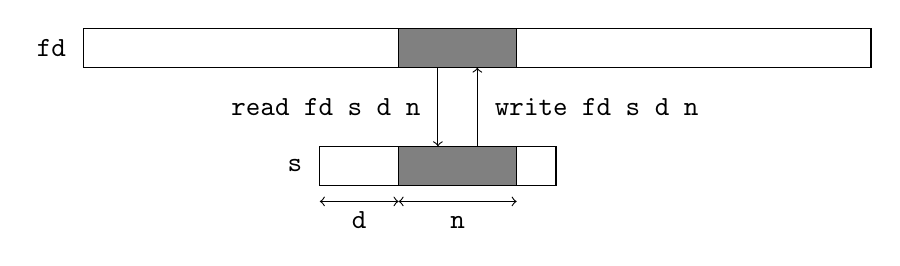
\begin{tikzpicture}[font={\ttfamily}]
\path[draw,fill=gray] (1,1.5) rectangle +(1.5, 0.5);
\path[draw] (-3,1.5) rectangle +(10, 0.5);
\node[anchor=east] at (-3.1,1.75) {fd};

\draw[->] (1.5, 1.5) to node [left=1mm] {read fd s d n} (1.5, 0.5);
\draw[<-] (2, 1.5) to node [right=1mm] {write fd s d n} (2, 0.5);

\path[draw,fill=gray] (1,0) rectangle +(1.5, 0.5);
\path[draw] (0,0) rectangle (3, 0.5);
\node[anchor=east] at (-0.1,0.25) {s};

\draw[<->] (0,-0.2) to node [below] {\phantom{n}d\phantom{n}} (1,-0.2);
\draw[<->] (1,-0.2) to node [below] {\phantom{d}n\phantom{d}} (2.5,-0.2);
\end{tikzpicture}
\end{myimage}
%


\ml+read+ or \ml+single_write+ return the number of bytes actually read or written. 

The reads and writes are started from the current position 
of the read/write. (If the file was opened in \ml+O_APPEND+ mode,
this position is the end of the file prior to any writes.) This 
position is advanced by the number of bytes read or written.

In the case of a write, the number of bytes actually written
is normally the number of bytes requested, but there are many
exceptions to this behaviour: (i) In the case where it is not possible
to write the bytes (for example, if the disk is full); (ii) When
the write is on a descriptor of files opened on a pipe or
a lock file placed in non-blocking input/output mode, the write
could turn out to be partial; And lastly, (iii){\ocaml}, which makes
a supplementary copy in a scratch buffer and writes on it, limits
the size of the buffer to a maximum value ( which is in general the
size used by the system for its own buffers) so as to avoid allowing
buffers of too large a size ; if the number of bytes to write is 
larger than this limit, then the write is necessarily partial 
in the same way as if the system did not have enough resources to
effect a complete write.

To work around the problem of buffer limits, {\ocaml} also provides
a function \ml+write+ which repeats many writes while there
are no write errors.  However, in case of error,
the function returns the error but we have no way of knowing 
the number of bytes actually written. Instead we should use \ml+single_write+ 
rather than \ml+write+ because it preserves atomicity.
(So that we know exactly what it has written) and it is more faithful to
the Unix system call (See likewise the implementation
of \ml+single_write+ described in the following chapter 
~\ref{single_write}).

In the following chapter, we shall see that when we write to a 
file descriptor which refers to a pipe or a lock file placed
in input/output blocking mode and which is then interrupted by a signal,
the call \ml+single_write+ returns an error \ml+EINTR+.
  

\begin{example} 
Assume \ml+fd+ is linked to an open descriptor which is writing. 
%
\begin{lstlisting}
write fd "Hello world!" 3 7
\end{lstlisting}
%
write the characters \quotes{"lo worl"} in the corresponding file,
and returns 7.
\end{example}

In the case of a read, it is possible that the number of bytes actually read may 
be less than the number of bytes requested. First case: When the end of a file
is near, that is to say, when the number of bytes between the current position
and the end of the file is less than the number of bytes requested. Specially,
when the current position is at the end of the file, \ml+read+ returns zero.
This convention \quotes{zero equals end of file} is also applied when reading
from a special (device) file or communication devices. For example, \ml+read+
on a terminal returns zero if one hits \ml+ctrl-D+ at the start of a line. 

Second case when the number of bytes read may be less than the number of bytes
requested:  When one reads from a special file such as a terminal, or
from a communication devices such as a pipe or a lock file. For example,
when we read from a terminal, \ml+read+ blocks until an entire line is available.
If the length of the line exceeds the number of bytes requested, \ml+read+ returns
the number of bytes requested. (This is the default behaviour of a terminal;
we can also place the terminal in character-by-character read mode instead of
line-by-line. See section~\ref{sec/speciaux} and the type \libtype{Unix}{terminal\_io}
for all the details.)

\begin{example} 
The following expression reads at most 100 characters from standard input
and returns the character string read. 
%
\begin{lstlisting}
let buffer = String.create 100 in
let n = read stdin buffer 0 100 in
  String.sub buffer 0 n
\end{lstlisting}
\end{example}

\begin{example} 

The function \ml+really_read+ below has the same interface as
\ml+read+, but makes additional read attempts if necessary 
to try to get the requested number of bytes. It triggers the exception \ml+End_of_file+
if it encounters the end of the file while doing this.

%
\begin{lstlisting}
let rec really_read fd buffer start length =
  if length <= 0 then () else
  match read fd buffer start length with
  | 0 -> raise End_of_file
  | r -> really_read fd buffer (start + r) (length - r);;
\end{lstlisting}
%
\end{example}

\section{Closing a descriptor}

The system call \syscall{close} closes the descriptor passed in as the argument.
%
\begin{listingcodefile}{tmpunix.mli}
val $\libvalue{Unix}{close}$ : file_descr -> unit
\end{listingcodefile}
%
Once a descriptor is closed, all attempts to read, write, or
to do anything whatever with the descriptor will fail. Descriptors should be
closed when they are no longer needed. In contrast to what occurs 
with the standard library \ml+Pervasives+, this is not obligatory.
In particular, it is not necessary to close descriptors in order to ensure
that attempted writes have been carried out: the writes made with 
\ml+write+ are immediately transmitted to the pipe. On the other hand,
the number of descriptors that a process can allow is limited by the pipe
(several hundreds to some thousands). Doing a \ml+close+ on an unused 
descriptor releases it, so that the process does not run out of descriptors.

\section{Complete example: file copy}
\label{ex/filecopy}
We will write a function \ml+file_copy+, with two arguments
\ml+f1+ and \ml+f2+,  which will copy the contents of the file named \ml+f1+
to a file named \ml+f2+.
%
\begin{listingcodefile}{file_copy.ml}
open Unix;;

let buffer_size = 8192;;
let buffer = String.create buffer_size;;

let file_copy input_name output_name =
  let fd_in = openfile input_name [O_RDONLY] 0 in
  let fd_out = openfile output_name [O_WRONLY; O_CREAT; O_TRUNC] 0o666 in
  let rec copy_loop () =
    match read fd_in buffer 0 buffer_size with
      0 -> ()
    | r -> ignore (write fd_out buffer 0 r); copy_loop () in
  copy_loop ();
  close fd_in;
  close fd_out;;
\end{listingcodefile}
%
\begin{codefile}{copy.ml}
open Unix
open File_copy
\end{codefile}
%
\begin{listingcodefile}{copy.ml}
let copy () =
  if Array.length Sys.argv = 3 then begin
    file_copy Sys.argv.(1) Sys.argv.(2);
    exit 0
  end else begin
    prerr_endline 
      ("Usage: " ^Sys.argv.(0)^ " <input_file> <output_file>");
    exit 1
  end;;

handle_unix_error copy ();;
\end{listingcodefile}
%

The core of the work is done in lines 6-15 of the function \ml+file_copy+.
We begin by opening a single read descriptor on the input file
and a single write descriptor on the output file.
If the output file already exists, it is truncated (option \ml+O_TRUNC+). 
If it does not exist it is created (option \ml+O_CREAT+), with
the permissions \ml+rw-rw-rw-+ modified through the creation mask. (
This is unsatisfactory: if we are copying an executable file, we would
like the copy to also be executable. We will see later how to 
attribute to a copy the same access permissions as the original.)
In Lines 9-13, in the function \ml+copy_loop+, we carry out the copy with character blocks of size 
\ml+buffer_size+  . We request a read of  \ml+buffer_size+
characters. If \ml+read+ returns zero, it means that we have reached 
the end of the input file and the copy is terminated. Otherwise, we write
the \ml+r+ bytes which we have read into the output file and start again.

Finally, we close the two descriptors. The main program
\ml+copy+ verifies that the program has received two arguments and passes them to the function
\ml+file_copy+.

While copying, all errors, such as for example
not being able to open the input file because it does not exist
or because the process does not have read permissions on the file or
further the failure of a write for lack of disk space,
result in an exception \ml+Unix_error+ which is propagated as far as the highest level 
of the program or is intercepted and displayed by
\ml+handle_unix_error+.

\begin{exercise} 
Add an option \ml+-a+ to the program, such that 
\ml+file_copy -a f1 f2+ appends the contents of \ml+f1+ to the end of
the file \ml+f2+ if \ml+f2+ exists. 
\end{exercise}
\begin{answer}
If the option \ml+-a+ is supplied, we need to do 
%
\begin{lstlisting}
openfile output_name [O_WRONLY; O_CREAT; O_APPEND] 0o666
\end{lstlisting}
%
instead of
%
\begin{lstlisting}
openfile output_name [O_WRONLY; O_CREAT; O_TRUNC] 0o666
\end{lstlisting}
%
The analysis of the option is left to the reader.
\end{answer}

\section{The cost of system calls.  The buffers.}

In the example \ml+file_copy+, the reads were made in blocks of 8192
bytes. Why not read byte by byte? Or megabyte by megabyte?
It is done for reasons of efficiency. Figure~\ref{fig/copy-speed}
shows the speed of copy, in bytes per second of the program
\ml+file_copy+, when we vary the size of the blocks (the variable
\ml+buffer_size+) from 1 byte to 8 megabytes the speed doubles each time.

For small block sizes, the copy speed is almost proportional
to the block size. While the amount of data transferred is the same
regardless of the size of the blocks. More specifically, the bulk of the 
time is not spent on transferring data but in the execution 
of the loop \ml+copy_loop+ and in the calls \ml+read+ and \ml+write+.
After measuring more finely, we see that it is the calls \ml+read+ and
\ml+write+ which take most of the time. We conclude then that a system 
call, while it does not have much to do (\ml+read+ read of one character),
takes a minimum of about 4 micro-seconds of time (on the machine that was
used for the test --a 2.8 GHz Pentium 4 ), let us say 1 to 10 microseconds.
For the input/output blocks of small size, the duration of the system call
is what predominates.  
  
For larger blocks, between 4K and 1M, speed is constant and 
optimal. Here, the time spent on system calls and the copy loop
is a little more than the time spent on the transfer of data.
For another part, the size of the buffer should be bigger than 
the size of the caches used by the system. And the time taken by the 
system to manage the transfer should predominate over the cost of 
a system call. \footnote{In fact, {\ocaml} limits the size of data
transfers to 16K (in the current version) in repeat multiple 
\ml+write+ system calls to carry out the complete transfer---see the discussion
in the section \ref{single_write}. But this limit is the at the same
point as the size of the system caches and is not observable.}

Finally, for very large blocks (8M and more) the speed is slightly
less than optimal.  Coming into play here is the time needed to
allocate the block and to assign pages to it as it goes along and
fills up real memory.

\begin{codefile}{speed_write.c}
#include <errno.h>
#include <string.h>
#include <caml/mlvalues.h>
#include <caml/memory.h>
#include <caml/signals.h>
#include <caml/unixsupport.h>

#define LONG_BUFFER_SIZE 9388608

CAMLprim value speed_write
        (value fd, value buf, value ofs, value len) {
  CAMLparam4(fd, buf, ofs, len);
  long numbytes;
  int ret = 0;
  char iobuf[LONG_BUFFER_SIZE];
  numbytes = Long_val(len);
  if (numbytes > LONG_BUFFER_SIZE) numbytes = LONG_BUFFER_SIZE;
  /* memmove (iobuf, &Byte(buf, Long_val(ofs)), numbytes); */
  /* enter_blocking_section(); */
  /* ret = write(Int_val(fd), iobuf, (int) numbytes); */
  ret = write(Int_val(fd), &Byte(buf, Long_val(ofs)), (int) numbytes);
  /* leave_blocking_section(); */
  if (ret == -1) uerror("write", Nothing);
  CAMLreturn (Val_int(ret));
}
\end{codefile}
%
\begin{codefile}{speed.ed}
f speed.ml
r file_copy.ml
3a
external speed_write :
   file_descr -> string -> int -> int -> int = "speed_write";;
.
/buffer_size/,/file_copy/c
let file_copy buffer_size input_name output_name =
  let buffer = String.create buffer_size in
.
/write/s/write/speed_write/
$a

let rec power n k = if k > 0 then n * power n (pred k) else 1;;
let copy () =
  if Array.length Sys.argv = 2 then begin
    let file = Sys.argv.(1) in
    let tmp = Filename.temp_file "foo" "bar" in
    let mega_octets = float (10 * (lstat file).st_size) /. 1e6 in
    (* put file in cache *)
    file_copy 10 file "/dev/null";
    for i = 23 downto 0 do 
      let start = let t = Unix.times() in t.tms_utime +. t.tms_stime in
      let block = power 2 i in
      for i = 1 to 10 do file_copy block file tmp done;
      let stop = let t = Unix.times() in t.tms_utime +. t.tms_stime in
      let time = stop -. start in
      let speed = mega_octets /. time in
      Printf.printf "%9d %.2f" block speed; 
      print_newline();
    done;
      exit 0
  end else begin
    prerr_endline ("Usage: " ^Sys.argv.(0)^ " <input_file> <output_file>");
    exit 1
  end;;

handle_unix_error copy ();;
.
wq
\end{codefile}
% $

\begin{myfigure}
\begin{myimage}[width="100\%"]
\begin{tikzpicture}[font=\tiny]
\pgfsetplotmarksize{0.8pt}
\draw plot[only marks,mark=*] file {data/speed-log.data};

% x-axis
\draw (0,-1) -- (7,-1);
\foreach \x in {0,...,7} { \draw (\x,-1) -- (\x,-0.95); };
\node at (0,-1.3) {\phantom{$^{2}$}1\phantom{$^{2}$}};
\node at (1,-1.3) {\phantom{$^{2}$}10\phantom{$^{2}$}};
\node at (2,-1.3) {\phantom{$^{2}$}100\phantom{$^{2}$}};
\foreach \x in {3,...,7} { \node at (\x,-1.3) {\phantom{$^{\x}$}10$^\x$}; };
\node at (8.5, -1.3) {Size (bytes)\phantom{1$^{1}$}};

% y-axis
\draw (-0.5,-0.5) -- (-0.5, 2.5);
\foreach \y in {-1,...,3} { \draw (-0.5,\y) -- (-0.45,\y); };
\node[anchor=east] at (-0.5,-1) {0.1\phantom{$^{3}$}};
\node[anchor=east] at (-0.5,0) {1\phantom{$^{3}$}};
\node[anchor=east] at (-0.5,1) {10\phantom{$^{3}$}};
\node[anchor=east] at (-0.5,2) {100\phantom{$^{3}$}};
\node[anchor=east] at (-0.5,3) {10$^{3}$};

\node[anchor=east] at (-0.5,3.5) {Speed (MB/s)};
\end{tikzpicture}
\end{myimage}
\caption{copy speed as a function of block size}
\label{fig/copy-speed}
\end{myfigure}

Moral:  A system call, even if it does very little work, costs
dearly---much more dearly than a normal function call: roughly,
from 2 to 20 microseconds for each system call, depending on the
the architecture. It is therefore important to avoid 
making system calls too frequently. If possible, read and write 
operations should be made in blocks of sufficient size and not
character by character.

In examples such as \ml+file_copy+, it is not difficult to do
input/ouput with large blocks. On the other hand, other types 
of programs are more naturally written with character by character
input (examples: Reading a line from a file, lexical analysis), and
displaying some characters at once (example: displaying a name). 
To satisfy the needs of these programs, most systems provide
input-output libraries with an additional layer of software between
the application and the operating system. For example, in {\ocaml} the
\ml+Pervasives+ module of the standard library defines the abstract
types \libtype{Pervasives}{in\_channel} and
\libtype{Pervasives}{out\_channel}, similar to file descriptors, and
functions on these types like \libvalue{Pervasives}{input\_char},
\libvalue{Pervasives}{input\_line},
\libvalue{Pervasives}{output\_char}, or
\libvalue{Pervasives}{output\_string}.  This layer uses buffers to
group sequences of character by character reads or writes into a
single read or write. This results in better performance for programs
that proceed character by character.  Moreover this additional layer
makes programs more portable~: we just need to implement this layer
with the system calls provided by another operating system to port the
all the programs that use this library on this new platform.

\section{Complete Example:  A small input-output library}

Here is an implementation of a part of the {\ocaml} \ml+Pervasives+ library to illustrate read/write
techniques by buffer. The interface is the following:
%
\begin{listingcodefile}{io.mli}
exception End_of_file

type in_channel
val open_in : string -> in_channel
val input_char : in_channel -> char
val close_in : in_channel -> unit

type out_channel
val open_out : string -> out_channel
val output_char : out_channel -> char -> unit
val close_out : out_channel -> unit
\end{listingcodefile}
%
We start with the \quotes{read} part. The abstract type 
\ml+in_channel+ is implemented as follows: 
%
\begin{listingcodefile}{io.ml}
open Unix;;

type in_channel =
  { in_buffer: string;
    in_fd: file_descr;
    mutable in_pos: int;
    mutable in_end: int };;
exception End_of_file
\end{listingcodefile}
%

The character string in the field \ml+in_buffer+ is literally the buffer.
The field \ml+in_fd+ is a file descriptor 
(Unix), opened on the file during the read. The field 
\ml+in_pos+ is the current position of the read cursor in the buffer .  The
field \ml+in_end+ is the number of valid characters in the buffer.
%
\begin{myimage}[width="85\%"]
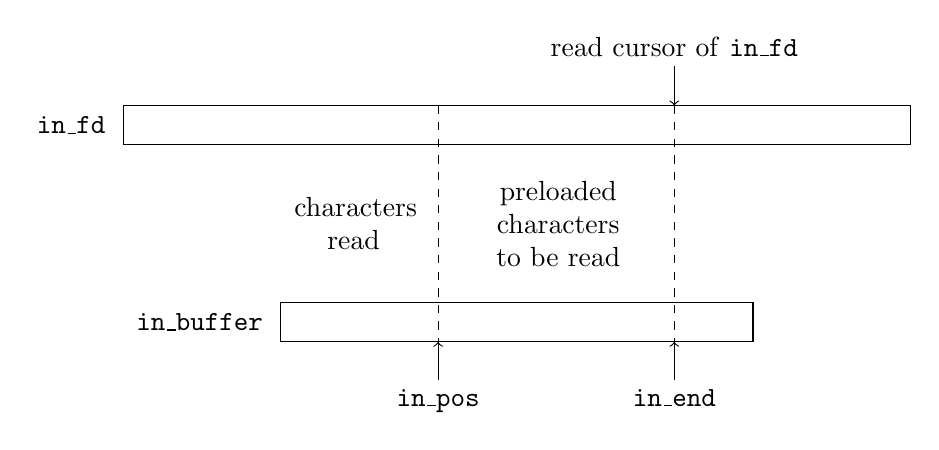
\begin{tikzpicture}
\path[draw] (-3,2.5) rectangle +(10, 0.5);
\node[anchor=east] at (-3.1,2.75) {\texttt{in\_fd}};
\draw[dashed] (1,3) to node [left=2mm,text width=1.5cm,text centered] 
 {characters read} (1,0);

\draw[dashed] (4,3) to node [left=1mm,text width=2.5cm,text centered] 
 {preloaded characters to be read} (4,0);

\path[draw] (-1,0) rectangle +(6, 0.5);
\node[anchor=east] at (-1.1,0.25) {\texttt{in\_buffer}};

\node (fdpos) at (4,3.75) {read cursor of \texttt{in\_fd}};
\draw[->] (fdpos.south) to (4,3);

\node (ipos) at (1,-0.75) {\texttt{\phantom{d}in\_pos\phantom{d}}};
\node (iend) at (4,-0.75) {\texttt{\phantom{p}in\_end\phantom{p}}};
\draw[->] (ipos.north) to (1,0);
\draw[->] (iend.north) to (4,0);
\end{tikzpicture}
\end{myimage}

The field \ml+in_pos+ and \ml+in_end+ will be modified in place during 
read operations ; we therefore call them  \ml+mutable+.
%
\begin{listingcodefile}{io.ml}
let buffer_size = 8192;;
let open_in filename =
  { in_buffer = String.create buffer_size;
    in_fd = openfile filename [O_RDONLY] 0;
    in_pos = 0;
    in_end = 0 };;
\end{listingcodefile}
%
At the opening of a file in read mode, we create a buffer of
reasonable size (large enough so not to make too many
system calls; small enough so as not to waste memory). We
then initialise the field \ml+in_fd+ with a Unix file descriptor
opened in read mode on the file in question. The 
buffer is initially empty (It does not contain any characters from the file); 
the field \ml+in_end+ is thus initialised to zero.
%
\begin{listingcodefile}{io.ml}
let input_char chan =
  if chan.in_pos < chan.in_end then begin
    let c =  chan.in_buffer.[chan.in_pos] in
      chan.in_pos <- chan.in_pos + 1;
      c
  end else begin
    match read chan.in_fd chan.in_buffer 0 buffer_size
    with 0 -> raise End_of_file
       | r -> chan.in_end <- r;
              chan.in_pos <- 1;
              chan.in_buffer.[0]
  end;;
\end{listingcodefile}
%

To read a character from \ml+in_channel+, we do one of two things. 
Where there is at least one character in the buffer;
that is to say, the field \ml+in_pos+ is less than the field 
\ml+in_end+. Then we return the next character in the buffer, that which
is in position  \ml+in_pos+, and we increment \ml+in_pos+. Where the buffer
is empty. We make a system call \ml+read+ to refill the 
buffer. If \ml+read+ returns zero, that means we have reached 
the end of the file; We then trigger the exception \ml+End_of_file+. Otherwise,
we put the number of characters read in the field \ml+in_end+. (We could 
have received less characters than we requested, and thus the buffer 
could have been partially refilled.) Then we return the first of the  
characters read.
%
\begin{listingcodefile}{io.ml}
let close_in chan =
  close chan.in_fd;;
\end{listingcodefile}
%
The closing of an \ml+in_channel+ is reduced to the closing of the underlying Unix descriptor. 

The \quotes{writing} part is very similar to the \quotes{reading} part. The 
only asymmetry is that the buffer now contains incomplete writes 
(characters that have already been buffered but not written to the file descriptor),
and not reads in advance (characters that have buffered, but not yet read).

\begin{myimage}[width="85\%"]
\begin{tikzpicture}
\path[draw] (-3,2.5) rectangle +(10, 0.5);
\node[anchor=east] at (-3.1,2.75) {\texttt{out\_fd}};
\draw[dashed] (1,3) to node [left=2mm,text width=1.5cm,text centered] 
 { caract�res �crits et vid�s} (1,0);

\draw[dashed] (4,3) to node [left,text width=2.5cm,text centered] 
 {caract�res �crits non vid�s} (4,0);

\path[draw] (1,0) rectangle +(4, 0.5);
\node[anchor=east] at (0.9,0.25) {\texttt{out\_buffer}};

\node (fdpos) at (1,3.75) {write cursor of \texttt{out\_fd}};
\draw[->] (fdpos.south) to (1,3);

\node (opos) at (4,-0.75) {\texttt{out\_pos}};
\draw[->] (opos.north) to (4,0);
\end{tikzpicture}
\end{myimage}
%
\begin{listingcodefile}{io.ml}
type out_channel =
  { out_buffer: string;
    out_fd: file_descr;
    mutable out_pos: int };;

let open_out filename =
  { out_buffer = String.create 8192;
    out_fd = openfile filename [O_WRONLY; O_TRUNC; O_CREAT] 0o666;
    out_pos = 0 };;

let output_char chan c =
  if chan.out_pos < String.length chan.out_buffer then begin
    chan.out_buffer.[chan.out_pos] <- c;
    chan.out_pos <- chan.out_pos + 1
  end else begin
    ignore (write chan.out_fd chan.out_buffer 0 chan.out_pos);
    chan.out_buffer.[0] <- c;
    chan.out_pos <- 1
  end;;

let close_out chan =
  ignore (write chan.out_fd chan.out_buffer 0 chan.out_pos);
  close chan.out_fd;;
\end{listingcodefile}
%
 
To write a character on an \ml+out_channel+, where the buffer 
is not full, it suffices to store the character in the buffer
in the position \ml+out_pos+, and to advance \ml+out_pos+; when 
the buffer is full, we empty the buffer with 
a call to \ml+write+, then we store the character to write at the beginning of 
the buffer.

When we close an \ml+out_channel+, we should not forget to dump  
the buffer contents (the characters between the positions 0 included and 
\ml+out_pos+ excluded) into the file. Otherwise, the writes 
made after the last dump will be lost.

\begin{exercise} 
Implement a function 
%
\begin{lstlisting}
val output_string : out_channel -> string -> unit
\end{lstlisting}
%
which behaves like a series of \ml+output_char+ on each 
character of the string, but is more efficient.
\end{exercise}
\begin{answer}

The idea is to copy the string to be output into the buffer. We need to 
take into account the case where there is not enough space in the buffer
(in that case the buffer needs to emptied), and also the case where the string is  
longer than the buffer can hold (in that case it is necessary to write it directly). 
Here is a possible solution. 
%
\begin{codefile}{ex2.ml}
open Unix;;
\end{codefile}
%
\begin{listingcodefile}{ex2.ml}
let output_string chan s =
  let avail = String.length chan.out_buffer - chan.out_pos in
  if String.length s <= avail then begin
    String.blit s 0 chan.out_buffer chan.out_pos (String.length s);
    chan.out_pos <- chan.out_pos + String.length s
  end
  else if chan.out_pos = 0 then begin
    ignore (write chan.out_fd s 0 (String.length s))
  end
  else begin
    String.blit s 0 chan.out_buffer chan.out_pos avail;
    let out_buffer_size = String.length chan.out_buffer in
    ignore (write chan.out_fd chan.out_buffer 0 out_buffer_size);
    let remaining = String.length s - avail in
    if remaining < out_buffer_size then begin
      String.blit s avail chan.out_buffer 0 remaining;
      chan.out_pos <- remaining
    end else begin
      ignore (write chan.out_fd s avail remaining);
      chan.out_pos <- 0
    end
  end;;
\end{listingcodefile}
%
\begin{codefile}{ex2.ml}
let ex2() = 
  if Array.length Sys.argv < 3 then begin 
     prerr_string "Usage: test <sources> <dest>"; 
     exit 2;
  end;
  let fdin = open_in Sys.argv.(1) in
  let fdout = open_out Sys.argv.(2) in
  prerr_endline "copying";
  try while true do output_char fdout (input_char fdin) done
  with End_of_file -> 
   prerr_endline "Done";
   output_string fdout "The end.\n";
   prerr_endline "Closing";
   close_out fdout;;

handle_unix_error ex2();;
\end{codefile}
%
\begin{codefile}{ex2.test}
./ex2.byte ex2.ml ex2.out
(cat ex2.ml; echo "C'est la fin.") | diff --brief - ex2.out
rm ex2.out
\end{codefile}
\end{answer}


\section{Positioning}

The system call \syscall{lseek} permits changing the current position of the read/write cursor.
%
\begin{codefile}{tmpunix.mli}
type seek_command = Unix.seek_command
\end{codefile}
%
\begin{listingcodefile}{tmpunix.mli}
val $\libvalue{Unix}{lseek}$ : file_descr -> int -> seek_command -> int
\end{listingcodefile}
%

The first argument that we need to place is the descriptor.
The second argument is the desired position. This is interpreted differently 
depending on the value of the third argument, which indicates the 
type of position desired:
%
\begin{mltypecases}
\mltypecase{SEEK\_SET} Absolute position. The second argument is 
the index into the file, in characters, to position the pointer at. The first character of a file 
is at position zero. 

\mltypecase{SEEK\_CUR} Position relative to the current position. 
The second argument is a displacement relative to the  
current position. This may be negative to move backwards or positive
to move forwards.

\mltypecase{SEEK\_END} Position relative to the end of file. The 
second argument is a displacement relative to the end of file.
This may be negative as well as positive.
\end{mltypecases}
%


The value returned by \ml+lseek+ is the absolute position of the read/write cursor 
(after it has actually been positioned).

An error is triggered if the absolute position requested is negative.
On the other hand, the position requested could well be located after
the end of file. Right after such a positioning, a  \ml+read+
returns zero (end of file reached); an \ml+write+ extends the file 
from the zero up to the position requested, then writes the supplied data. 

\begin{example} 
To position the cursor on the 1000th character of a file:
%
\begin{lstlisting}
lseek fd 1000 SEEK_SET
\end{lstlisting}
%
To rewind by one character:
%
\begin{lstlisting}
lseek fd (-1) SEEK_CUR
\end{lstlisting}
%
To find the size of a file:
%
\begin{lstlisting}
let file_size = lseek fd 0 SEEK_END in ...
\end{lstlisting}
\end{example}

For descriptors opened in \ml+O_APPEND+ mode, the read/write cursor is 
automatically placed at the end of the file before each write. 
Thus the call \ml+lseek+ is useless for writing 
on such a descriptor. On the other hand, it is well taken into account
by the read. 

The behaviour of \ml+seek+ is unpredictable on certain type of files
for which direct access is meaningless: communication devices (pipes, lock files),
but also most special files (peripherals), such as for example the terminal.
For most implementations of Unix, an \ml+lseek+ on such files 
is simply ignored:  The read/write cursor is positioned 
but read/write operations ignore it.
In some implementations, \ml+lseek+ on a pipe or on a lock file
triggers an error.

\begin{exercise}

The command \ml+tail+ displays the $n$ last lines of a file.
How should it be efficiently implemented if the file in question is
a normal file? How should it be done to cope with other types of files?
How to add the option \ml+-f+ (cf. \ml+man tail+) ? .
\end{exercise}
\begin{answer}
The naive implementation of \ml+tail+ is to read the file
sequentially from the beginning keeping the last $n$ lines read in
a circular buffer. When we reach the end of file, we display the buffer. 
When the data comes from a pipe or a special file which
does not implement \ml+lseek+, there is no better way.
On the other hand, if the data is coming from a normal file,
it would be better to read the file starting from the end: with 
\ml+lseek+, we read the last 4096 characters:  We scan them for 
the end of line;hr.  If there are at least $n$, we output and display
the corresponding lines.  Otherwise, we start again with the preceding
4096 characters, etc.

To add the option \ml+-f+,it suffices to at once display the last 
$n$ lines, to position the cursor at the end of the file and to
attempt to read (through \ml+read+) starting from it. If \ml+read+
succeeds to read something, we display it immediately and begin again.
If \ml+read+ returns 0, we wait a little (\ml+sleep 1+) then 
try again. 
\end{answer}

\section{Operations specific to certain file types}

In Unix, data communication is done via file descriptors representing
either permanent files (files, peripherals) or volatile ones (pipes
and sockets, see chapters~\ref{sec/pipes} and \ref{sec/sockets}). File
descriptors provide a uniform and media-independent interface for data
communication. Of course the actual implementation of the operations
on a file descriptor depends on the underlying media.

However this uniformity breaks when one needs to access all the
features provided by a given media. General operations (opening,
writing, reading, \etc) remain uniform on most descriptors but even,
on certain special files, these may have an ad-hoc behaviour defined
by the kind of peripheral and its parameters. There are also
operations that work only with certain kind of media.

\subsection*{Normal files}

We can shorten an ordinary file through the system calls
\syscall{truncate} and \syscall{ftruncate}.
%
\begin{listingcodefile}{tmpunix.mli}
val $\libvalue{Unix}{truncate}$  : string -> int -> unit
val $\libvalue{Unix}{ftruncate}$ : file_descr -> int -> unit
\end{listingcodefile}
%

The first argument is the file to truncate (specified either by its
name or by a descriptor open on the file). The second argument is the
desired size. All the data starting from this position is lost.

\subsection*{Symbolic links}

Most of the the operations on files \quotes{follow} symbolic 
links: that is to say, they are applied to files to which 
the symbolic link points, and not on the symbolic link 
itself. Examples: \indexvalue{openfile}, \indexvalue{stat},
\indexvalue{truncate}, \indexvalue{opendir}. We have two 
operations, \syscall{symlink} and \syscall{readlink} on symbolic
links:
%
\begin{listingcodefile}{tmpunix.mli}
val $\libvalue{Unix}{symlink}$  : string -> string -> unit
val $\libvalue{Unix}{readlink}$ : string -> string
\end{listingcodefile}
%
The call \ml+symlink f1 f2+ creates the file \ml+f1+ as the symbolic 
link of \ml+f2+ (like the command \ml+ln -s f1 f2+). The call 
\ml+readlink+ returns the content of a symbolic link, that is to say a 
the name of the file to which it points.

\subsection*{Special files}
\label{sec/speciaux}

Special files may be of type \quotes{character} or of 
type \quotes{block}.  The first are for reading and writing characters: we cannot 
read or write characters expect in sequence. These character devices are 
typically terminals, the peripherals are, printers,
etc. The second, typically disks, are a permanent or temporary resource:
characters are read in blocks given in absolute form or relative with respect to the current position
Among the special files, we may distinguish:
\begin{mltypecases}
\mltypecase{/dev/null} This is the black hole which swallows everything 
that is put into it and from which nothing comes out. Extremely useful for ignoring  
the results of a process: we redirect its output to \ml+/dev/null+ (see the
chapter \ref{sec/pipes}).

\mltypecase{/dev/tty*}  These are the terminals.

\mltypecase{/dev/pty*} These are the pseudo-terminals: They 
are not real terminals but provide the
same interface.

\mltypecase{/dev/sd*}
\mltypecase{/dev/hd*} These are the disks.  

\mltypecase{/proc} Under Linux, enable reading and writing of some  
system parameters organized as a file system.
\end{mltypecases}

The special files have a behaviour sufficient variable in response
to system calls generated on files. Most special files 
(terminals, tape drives, disks, \ldots) follow 
\ml+read+ and \ml+write+ in the obvious manner (but sometimes with 
restrictions on the number of bytes written or read). Many 
special files ignore \indexvalue{lseek}.

In most system generated calls, special files which 
correspond to the  peripherals should be able to have dynamic parameters 
or commands. Examples of such possibilities: To 
rewind the tape, rewind or fast forward; for a terminal 
terminal, choice of line editing mode, special characters 
, serial connection parameters (speed, parity, etc).
These operations are made in Unix through the system call  
\syscall{ioctl} which group together all the particular cases. However, this
system call is not provided by {\ocaml}... because it is  
ill-defined and cannot be treated in a uniform way. 

\subsubsection{Terminals}
\label{sec/termio}


The terminals (or  pseudo-terminals) are a particular 
case of special files of type character for which 
{\ocaml} gives access to the configuration. The call \syscall{tcgetattr}
takes as an argument a file descriptor open on the special file 
in question and returns a structure of type
\ml+terminal_io+ which describe the state of the terminal
represented by the file according to the standard  \textsc{posix}.
%
\begin{codefile}{tmpunix.mli}
type terminal_io = Unix.terminal_io
\end{codefile}
%
\begin{lstlisting}
type $\libtype{Unix}{terminal\_io}$ = 
  { c_ignbrk : bool; c_brk_int : bool; ...;  c_vstop : char }
\end{lstlisting}
%
\begin{listingcodefile}{tmpunix.mli}
val $\libvalue{Unix}{tcgetattr}$ : file_descr -> terminal_io
\end{listingcodefile}
%
This structure may be modified then passed to the function 
\syscall{tcsetattr} to change the attributes of the peripheral.
%
\begin{codefile}{tmpunix.mli}
type setattr_when = Unix.setattr_when
\end{codefile}
%
\begin{listingcodefile}{tmpunix.mli}
val $\libvalue{Unix}{tcsetattr}$ : file_descr -> setattr_when -> terminal_io -> unit
\end{listingcodefile}
%
The first argument is the file descriptor of the peripheral. 
The last argument is a structure of type 
\ml+tcgetattr+ describing the parameters of the peripheral such that are  
needed for setup.  The second argument is a flag of the type enumeration.
\ml+setattr_when+ indicating the moment from which the change 
should take effect: immediately (\ml+TCSANOW+), after having transmitted
all written data (\ml+TCSADRAIN+) or after having read all the data 
received (\ml+TCAFLUSH+).  The choice \ml+TCSADRAIN+ is
recommended for changing the write parameters and \ml+TCSAFLUSH+
for modifying the read parameters. 

\begin{example}
During the reading of a password, there should be no echo  
of the characters keyed by the user if the flow of standard input is
connected to a terminal or pseudo-terminal.
%
\begin{codefile}{passwd.ml}
open Unix;;
\end{codefile}
%
\begin{listingcodefile}{passwd.ml}
let read_passwd message = 
  match
    try 
      let default = tcgetattr stdin in
      let silent = 
        { default with 
          c_echo = false; 
          c_echoe = false; 
          c_echok = false; 
          c_echonl = false; 
        } in
      Some (default, silent) 
    with _ -> None
  with 
  | None -> input_line Pervasives.stdin
  | Some (default, silent) -> 
      print_string message; 
      flush Pervasives.stdout;
      tcsetattr stdin TCSANOW silent;
      try 
        let s = input_line Pervasives.stdin in 
        tcsetattr stdin TCSANOW default; s
      with x -> 
        tcsetattr stdin TCSANOW default; raise x;;
\end{listingcodefile}
%

The \ml+read_passwd+ function begins by recovering the default value  
of the terminal associated with \ml+stdin+ and constructing 
a modified version in which the characters do not have echo.  
In case of failure, when the input stream is not a terminal,
it is enough to read a line. Otherwise we display
a message, we change the terminal, we read the response and reset the  
terminal into its normal state. Care has to be taken to set
the terminal back to its normal state after a read failure.
\end{example}
%
Sometimes a program needs to launch another linked to its
input stream from a terminal (or pseudo-terminal).  {\ocaml} does not
supply any support for this \footnote {The Cash library
~\cite {Cash} supplies such functions.} so it is necessary to manually
look for an unused pseudo-terminals  (in general, they are files 
with names in the form of \ml+/dev/tty[a-z][a-f0-9]+) and find one of 
these files which has not already been opened, open it and launch  
the application with this file in the input stream.

Four other functions allow control of the stream (flush data on hold,
wait for end of transmission, restart communication). 
%
\begin{listingcodefile}{tmpunix.mli}
val $\libvalue{Unix}{tcsendbreak}$ : file_descr -> int -> unit
\end{listingcodefile}
%
The function  \syscall{tcsendbreak} sends an interrupt to the 
peripheral. Its second argument is the length of the interrupt
(\ml+0+ is interpreted as the default value for the 
peripheral).
%
\begin{listingcodefile}{tmpunix.mli}
val $\libvalue{Unix}{tcdrain}$ : file_descr -> unit
\end{listingcodefile}
%
The function \syscall{tcdrain} waits for all the data written to be 
transmitted.
%
\begin{codefile}{tmpunix.mli}
type flush_queue = Unix.flush_queue
\end{codefile}
%
\begin{listingcodefile}{tmpunix.mli}
val $\libvalue{Unix}{tcflush}$ : file_descr -> flush_queue -> unit
\end{listingcodefile}
%
Following the value of the flag passed in the second argument, the function
\syscall{tcflush} abandons the data written but not yet transmitted
(\ml+TCIFLUSH+), or the data received but not yet read 
(\ml+TCOFLUSH+) or both (\ml+TCIOFLUSH+).
%
\begin{codefile}{tmpunix.mli}
type flow_action = Unix.flow_action
\end{codefile}
%
\begin{listingcodefile}{tmpunix.mli}
val $\libvalue{Unix}{tcflow}$ : file_descr -> flow_action -> unit
\end{listingcodefile}
%

Following the value of the flag passed in the second argument, the function 
\syscall{tcflow} suspends the emission (\ml+TCOOFF+), restarts 
the emission (\ml+TCOON+), sends a control character \textsc{stop}
or \textsc{start} to request that the transmission be suspended
(\ml+TCIOFF+) or restarted (\ml+TCION+).
%
\begin{listingcodefile}{tmpunix.mli}
val $\libvalue{Unix}{setsid}$ : unit -> int
\end{listingcodefile}
%
The function \syscall{setsid} puts the process in a new
session and detaches it from the terminal.

\section{Locks on files}

Two processes may modify the same file in parallel at the risk
of some writes colliding with others. In some cases,the open
in \ml+O_APPEND+ mode allows these collisions to be managed, for example,
in the case of a \ml+log+ file where it suffices to write the 
information always at the end of the file.   But this mechanism
does not resolve the general case where the writes are at a prior 
arbitrary positions, for example, when a file represents a
database. It then becomes necessary for all the processes utilizing this file
to collaborate together so as not to step on each others toes.
A lock on the file is always possible by creating an auxiliary lock file
(see page \pageref{page/lock}). The system call 
\syscall{lockf} which does not lock more than a part of the file
allows a very accurate synchronization.
%
\begin{codefile}{tmpunix.mli}
type lock_command = Unix.lock_command
\end{codefile}
%
\begin{listingcodefile}{tmpunix.mli}
 val $\libvalue{Unix}{lockf}$ : file_descr -> lock_command -> int -> unit
\end{listingcodefile}


\section{Complete example: recursive copy of files}
\label{sec/copyrec}

We will extend the function \ml+file_copy+ (section~\ref{ex/filecopy})
to copy symbolic links and directories in addition to normal files. 
In the case of directories, we need copy their contents recursively.

We begin by retrieving the function \ml+file_copy+ in the example of the same name given 
for copying normal files (page~\pageref{ex/filecopy}). 
\begin{lstlisting}
open Unix
...
let file_copy input_name output_name =
...
\end{lstlisting}
The function \ml+set_infos+ below modifies the owner, the  
access rights and  the last dates of access/last modification
of a file. Its purpose is to preserve this information during the copy.

%
\begin{codefile}{copy_rec.ml}
open Unix;;
open File_copy;;
\end{codefile}
%
\begin{listingcodefile}{copy_rec.ml}
let set_infos filename infos =
  utimes filename infos.st_atime infos.st_mtime;
  chmod filename infos.st_perm;
  try
    chown filename infos.st_uid infos.st_gid
  with Unix_error(EPERM,_,_) -> ()
\end{listingcodefile}
%
The system call \ml+utime+ modifies the dates of access and 
modification.  We use \ml+chmod+ and \ml+chown+ to re-establish 
the access rights and the owner. For normal users, there are  
a certain number of cases where  \ml+chown+ will fail with an error
\quotes{permission denied}.  We trap this error and ignore it.

Here's the main recursive function. 
\begin{listingcodefile}{copy_rec.ml}
let rec copy_rec source dest =
  let infos = lstat source in
  match infos.st_kind with
    S_REG ->
      file_copy source dest;
      set_infos dest infos
  | S_LNK ->
      let link = readlink source in
      symlink link dest
  | S_DIR ->
      mkdir dest 0o200;
      Misc.iter_dir
        (fun file ->
          if file <> Filename.current_dir_name 
              && file <> Filename.parent_dir_name 
          then 
            copy_rec
              (Filename.concat source file)
              (Filename.concat dest file))
        source;
      set_infos dest infos
  | _ ->
      prerr_endline ("Can't cope with special file " ^ source)
\end{listingcodefile}

We begin by reading the information from the source file. If this is a 
normal file, we copy its contents with \ml+file_copy+, then its 
information with \ml+set_infos+. If it is a symbolic link, we read
where it points to, and we create a link which points to the same 
object.  If it is a directory, we create a directory as the
destination, then we read the directory entries in the source (ignoring
the entries which are about the source  \ml+Filename.current_dir_name+
or its parent directory \ml+Filename.parent_dir_name+, which we should 
certainly not copy), then we recursively call \ml+copy+ for 
each entry.  We ignore the other type of files, and include a  
warning.

The main program is relatively straight forward:
%
\begin{codefile}{copyrec.ml}
open Unix
open Copy_rec
\end{codefile}
%
\begin{listingcodefile}{copyrec.ml}
let copyrec () =
  if Array.length Sys.argv <> 3 then begin
    prerr_endline ("Usage: " ^Sys.argv.(0)^ " <source> <destination>");
    exit 2
  end else begin
    copy_rec Sys.argv.(1) Sys.argv.(2);
    exit 0
  end
;;
handle_unix_error copyrec ();;
\end{listingcodefile}

\begin{exercise} 
\label{ex/copyrec}
Intelligently copy hard links. As is described in the following,
\ml+copyrec+ creates $n$ duplicates of the same file which appears under $n$
different names in the hierarchy of files to copy. Try to detect this
situation and try not to copy the file more than once. 
Make hard links in the target hierarchy.
\end{exercise}

\begin{answer}
It is necessary to keep a table of source files that have already been copied, for which  
the tuple \ml+(st_dev, st_ino)+ for each source file corresponds with  
the name of its destination file. For each copy, we look up this
table to see if a source file with the same tuple
\ml+(st_dev,st_ino)+ had already been copied; if yes, we make a hard link  
to the target file, instead of repeating the copy. To minimize 
the size of this table, we can insert only the files 
which have more than one name, that is to say those where \ml+st_nlink > 1+.
%
\begin{codefile}{copyrec_ex.ml}
open File_copy
open Copy_rec
open Sys
open Unix
\end{codefile}
%
\begin{listingcodefile}{copyrec_ex.ml}
let copied_files = (Hashtbl.create 53 : ((int * int), string) Hashtbl.t)

let rec copy source dest =
  let infos = lstat source in
  match infos.st_kind with
    S_REG ->
      if infos.st_nlink > 1 then begin
        try
          let dest' = 
            Hashtbl.find copied_files (infos.st_dev, infos.st_ino)
          in link dest' dest
        with Not_found ->
          Hashtbl.add copied_files (infos.st_dev, infos.st_ino) dest;
          file_copy source dest;
          set_infos dest infos
      end else begin
        file_copy source dest;
        set_infos dest infos
      end
\end{listingcodefile}
\begin{lstlisting}
  | S_LNK -> ...
\end{lstlisting}
\begin{codefile}{copyrec_ex.ml}
| _ -> ()
\end{codefile}
\end{answer}

\section{Example: {\normalfont\texttt{T}}ape {\normalfont\texttt{AR}}chive}

The \ml+tar+ format (for \ml+t+ape \ml+ar+chive) allows us to represent 
a group of files in one file.  (In addition it allows us to store 
an entire file hierarchy on a tape.)  This is thus
in a way a mini file system. 

In this section we describe a group of functions which 
allows the reading and writing of archives in the \ml+tar+ format. The  
first part which is completely described, consists of writing a function
\ml+readtar+ such that  \ml+readtar a+ displays a list of files 
contained in the archive~\ml+a+  and \ml+a f+ displaying the contents of  
a file \ml+f+ contained within the archive \ml+a+. We leave as an 
exercise the problem of extracting all the files contained in an archive
as well as generating an archive starting from a group of files.

\paragraph{Description of format}

A \ml+tar+ archive is a set of records,each 
record represents a file.  A record is composed of a header
which encodes the information about the file (its name, type, size, owner \etc) 
and the contents of the file.
The header consists of a block (512 bytes) as shown in the figure~\ref {fig/tar}.
\begin{mytable}
\begin{tabular}{rrlll}
Offset & Length & Code Type & Name & Description \\
\hline
  0&   100 & string  &  \ml+name+   & file name \\
100&     8 & octal   &  \ml+perm+   & file access modes\\
108&     8 & octal   &  \ml+uid+    & \textsc{id} of user\\
116&     8 & octal   &  \ml+gid+    & \textsc{id} of group of the user\\
124&    12 & octal   &  \ml+size+   & file size (in bytes)\\
136&    12 & octal   &  \ml+mtime+  & Date of last modification\\
148&     8 & octal   &  \ml+checksum+ & Header checksum \\
156&     1 &character&  \ml+kind+   & File type  \\
157&   100 & octal   &\emph{\ml+link+}   & Link\\
257&     8 & string  &  \ml+magic+  & Signature (\ml+"ustar\032\032\0"+)\\
265&    32 & string  &  \ml+user+   & Name of user\\
297&    32 & string  &  \ml+group+  & Name of user's group\\
329&     8 & octal   &\emph{\ml+major+}  & Peripheral major number\\
337&     8 & octal   &\emph{\ml+minor+}  & Peripheral minor number\\
345&   167 &         &         & Padding
\end{tabular}
\medskip
\begin{flushleft}\small
\textbf{Note.}\quad Field lengths are in number of bytes. All
fields are encoded with character strings terminated with the null character \ml+'\000'+; excepting the field \ml+kind+ and \ml+size+
(\ml+'\000'+ optional).
\end{flushleft}
\caption {Header structure}
\label{fig/tar}
\end{mytable}

The contents are represented by a number of whole blocks following the header. 
The records are given one after another. If necessary, the file is padded
with empty blocks in order to reach a minimum of 20 blocks. 

As the archives are also designed to be written on unreliable media
and retrieved many years later, the header contains a \ml+checksum+ field
which allows the archives to be found when the header is damaged (or to
use more than one file as an archive.) Its value is the sum of character
codes in the header (from this, we hypothesize that the 
\ml+checksum+ field which is not yet calculated consists of blanks
terminated by the null character). 

The \ml+kind+ field encodes the file type in a byte.
Significant values are the characters indicated in the table below. \footnote
{This field can also take different values to encode pathological cases, for example,
when the value of a field exceeds the place reserved for it in the header or
in the extensions of the \ml+tar+ command.}: 
\begin{center}
\begin{tabular}{cccccccc}
\ml+'\0'+ ou \ml+'0'+ & 
\ml+'1'+ & \ml+'2'+ &\ml+'3'+ & \ml+'4'+ & \ml+'5'+ & \ml+'6'+ & \ml+'7'+\\
\hline
\ml+REG+ & 
\ml+LINK+ & 
\ml+LNK+ & 
\ml+CHR+ & 
\ml+BLK+ & 
\ml+DIR+ & 
\ml+FIFO+ &
\ml+CONT+
\end{tabular}
\end{center}
Most of the cases correspond to the \ml+st_link+ type of Unix file.
The case \ml+LINK+ represents hard links: These have 
the same node (\emph{inode}) but are accessible through two different paths.
In this case,the link must lead to another
file already defined within the archive. The case \ml+CONT+ represents an 
ordinary file, but which is represented by a contiguous memory zone
(this is a feature of some types of file systems, we can then treat it
like an ordinary file).  The field 
\emph{\ml+link+} represents the link when the value of \ml+kind+ equals \ml+LNK+ or 
\ml+LINK+.  The fields \emph{\ml+major+} and \emph{\ml+minor+}
contain the major and minor numbers of the peripheral in the case 
where the value of the field \ml+kind+ equals \ml+CHR+ or \ml+BLK+. These three fields are
not used in other cases.

The value of the field \ml+kind+ is naturally represented by a concrete type;
the header by a record:
%
\begin{codefile}{tarlib.ml}
open Unix;;
\end{codefile}
%
\begin{listingcodefile}{tarlib.ml}
type kind =
  | REG | LNK of string | LINK of string | CHR of int * int 
  | BLK of int * int | DIR | FIFO | CONT

type header = 
    { name : string; perm : int; uid : int; gid : int; size : int; 
      mtime : int; kind : kind; user : string; group : string } 
\end{listingcodefile}

\paragraph {Reading a header}
Reading a header is not very interesting, but 
cannot be ignored.
%
\begin{listingcodefile}{tarlib.ml}
exception Error of string * string
let error err mes = raise (Error (err, mes));;
let handle_error f s = 
  try f s with 
  | Error (err, mes) -> 
      Printf.eprintf "Error: %s: %s" err mes;
      exit 2
        
let substring s offset len = 
  let max_length = min (offset + len + 1) (String.length s) in
  let rec real_length j =
    if j < max_length && s.[j] <> '\000' then real_length (succ j) 
    else j - offset in
  String.sub s offset (real_length offset);;

let integer_of_octal nbytes s offset =
  let i = int_of_string ("0o" ^ substring s offset nbytes) in
  if i < 0 then error "Corrupted archive" "integer too large" else i;;

let kind s i =
  match s.[i] with
  | '\000' | '0' -> REG
  | '1' -> LINK (substring s (succ i) 99)
  | '2' -> LNK (substring s (succ i) 99)
  | '3' -> CHR (integer_of_octal 8 s 329, integer_of_octal 8 s 329)
  | '4' -> BLK (integer_of_octal 8 s 329, integer_of_octal 8 s 337)
  | '5' -> DIR | '6' -> FIFO | '7' -> CONT
  | _ -> error "Corrupted archive" "kind"
        
let header_of_string s =
  { name = substring s 0 99;
    perm = integer_of_octal 8 s 100;
    uid = integer_of_octal 8 s 108;
    gid = integer_of_octal 8 s 116;
    size = integer_of_octal 12 s 124; 
    mtime = integer_of_octal 12 s 136;
    kind = kind s 156;
    user = substring s 265 32;
    group = substring s 297 32; }
    
let block_size = 512;;
let total_size size = 
  block_size + ((block_size -1 + size) / block_size) * block_size;;    
\end{listingcodefile}
%
The end of the archive is marked either at the end of the file where
a new record would begin, or on a complete, but empty, block. Thus to
read the header we need to try to read a block which should be either
empty or complete. To read an entire block we reuse the
\ml+really_read+ function we defined above. The end of file should not
be reached when we try to read a block.
%
\begin{codefile}{tarlib.ml}
let rec really_read fd buffer start length =
  if length <= 0 then () else
    match read fd buffer start length with
      0 -> raise End_of_file
    | r -> really_read fd buffer (start+r) (length-r);;
\end{codefile}
%
\begin{listingcodefile}{tarlib.ml}
let buffer_size = block_size;;
let buffer = String.create buffer_size;;

let end_of_file_error() = 
  error "Corrupted archive" "unexpected end of file"
let without_end_of_file f x = 
  try f x with End_of_file -> end_of_file_error()
      
let read_header fd = 
  let len = read fd buffer 0 buffer_size in
  if len = 0 ||  buffer.[0] = '\000' then None
  else begin
    if len < buffer_size then 
      without_end_of_file (really_read fd buffer len) (buffer_size - len);
    Some (header_of_string buffer)
  end;;
\end{listingcodefile}

\paragraph{Reading an archive}
To carry out any operation in an archive, it is necessary to read the group of
header records in order 
at least until those necessary to carry out the operation are found.
By default, it suffices to read the header of each record without
having to read the contents. Often it suffices to read the contents
of the record that we searched for or to read the content after finding
the previous record.  For this reason, it is necessary to keep information 
on the position of each record in the archive in addition to each header. 
We will use the following type for records:
%
\begin{listingcodefile}{tarlib.ml}
type record = { header : header; offset : int; descr : file_descr };;
\end{listingcodefile}
%
We will now write a general iterator which will read the 
records (without their contents) and will store them.
However, to maintain greater generality, we will remain at an abstract level compared  
to the storage function \ml+f+ (which can also add records to
those already read, print them, discard them, \etc).   
%
\begin{listingcodefile}{tarlib.ml}
let fold f initial fd  =
  let rec fold_aux offset accu = 
    ignore (without_end_of_file (lseek fd offset) SEEK_SET);
    match without_end_of_file read_header fd with
      Some h -> 
        let r = 
          { header = h; offset = offset + block_size; descr = fd } in
        fold_aux (offset + total_size h.size) (f r accu) 
    | None -> accu in
  fold_aux 0 initial;;
\end{listingcodefile}
%

The function \ml+fold_aux+ starts from a position  \ml+offset+ with a 
partial result \ml+accu+. It works by placing itself at position 
\ml+offset+, which should be the beginning of the record, reading
the header, constructing the record \ml+r+ then starts again at the end  
of the record with the new result \ml+f r accu+ (less
partial).  It stops when the header is empty which signifies
that it has arrived at the end of the archive.

\paragraph{Display of the list of records of an archive}
It suffices simply to display the group of records as we 
go along without keeping them: 
\begin{listingcodefile}{tarlib.ml}
let list tarfile =
  let fd = openfile tarfile [ O_RDONLY ] 0o0 in
  let add r () = print_string r.header.name; print_newline() in
  fold add () fd; 
  close fd
\end{listingcodefile}


\paragraph{Displaying the contents of a file in an archive}
The function \ml+readtar a f+ must search for the file with the name \ml+f+
in the archive and display it if it is a regular file.  Further, a
path \ml+f+ of the archive, which is a hard link and represents a path 
\ml+g+ of the archive, is followed and the contents of \ml+g+ are displayed: In 
effect, it is appropriate that \ml+f+ and \ml+g+ are represented differently in the 
final archive ( the one is a hard link to the other) they represent
exactly the same file at its creation. The fact that \ml+g+  is a
link to \ml+f+ or the converse depends uniquely on the order in which the 
files are traversed at the creation of the archive.  For the 
moment we will not follow symbolic links.

The main work resolving hard links is carried out by the two
following, recursively defined functions.
\begin{listingcodefile}{tarlib.ml}
let rec find_regular r list = 
  match r.header.kind with
  | REG | CONT -> r
  | LINK name -> find_file name list
  | _ -> error r.header.name "Not a regular file" 
and find_file name list = 
  match list with 
    r :: rest -> 
      if r.header.name = name then find_regular r rest
      else find_file name rest
  | [] -> error name "Link not found (corrupted archive)";;
\end{listingcodefile}
The function \ml+find_regular+ finds the regular file corresponding 
to a record (its first) argument.  If this is a regular file
it succeeds. If this is a special file 
or a symbolic link it fails.  In the remaining case of a hard link: The
function searches for the link in the list of records of the archive (second argument)  
by calling the function  \ml+find_file+.

Once the record is found there is nothing more to do except to display
its contents. This operation is strongly reminiscent of the function 
\ml+file_copy+, once the descriptor is positioned at the beginning of the file
in the archive. 
\begin{listingcodefile}{tarlib.ml}
let copy_file file output = 
  ignore (lseek file.descr file.offset SEEK_SET);
  let rec copy_loop len =
    if len > 0 then
      match read file.descr buffer 0 (min buffer_size len) with
        0 -> end_of_file_error()
      | r -> ignore (write output buffer 0 r); copy_loop (len-r) in
  copy_loop file.header.size
\end{listingcodefile}

The only thing left to do is to combine the previous three.
\begin{listingcodefile}{tarlib.ml}
exception Done
let find_and_copy tarfile filename =
  let fd = openfile tarfile [ O_RDONLY ] 0o0 in
  let found_or_collect r accu = 
    if r.header.name = filename then begin 
      copy_file (find_regular r accu) stdout;
      raise Done
    end else r :: accu in
  try 
     ignore (fold found_or_collect [] fd); 
     error "File not found" filename
  with
  | Done -> close fd 
\end{listingcodefile}
We read the records in the archive (but not their contents)
until we find a record with the target name. We call the function
\ml+find_regular+ to search the list of read records to find that one
which actually contains the file. 
The second, subsequent search will always succeed if the archive
is well-formed. In contrast the first, preceding search will fail 
if the record is not in the archive.  We need to take care to
distinguish errors due to a corrupt archive from those resulting
from an unproductive search.

And here is the main function which implements the function \ml+readtar+:
\begin{codefile}{readtar.ml}
open Unix
open Tarlib
\end{codefile}
\begin{listingcodefile}{readtar.ml}
let readtar () =
  let nargs = Array.length Sys.argv in 
  if nargs = 2 then list Sys.argv.(1)
  else if nargs = 3 then find_and_copy Sys.argv.(1) Sys.argv.(2)
  else 
    prerr_endline ("Usage: " ^Sys.argv.(0)^ " <tarfile> [ <source> ]");;

handle_unix_error (handle_error readtar) ();;
\end{listingcodefile}

\begin{exercise}
\label{ex/readtar}
Extend the function \ml+readtar+ so that it follows symbolic links, 
that is to say, so that it displays the file's contents 
if the archive had extracted it beforehand and if the file 
corresponds to a file in the archive.

Behind the apparent trivial appearance of this generalisation are hidden 
some difficulties, for the symbolic links are file paths some of which
may not correspond exactly with the paths in the archive which clearly
point outside the archive (they may contain the path \ml+..+). Further, symbolic
links may represent directories (which is not allowed for hard links).
\end{exercise}
\begin{answer}
A  sufficiently simple solution consists of simulating the effect of the extraction 
by creating in a graph an image of the file hierarchy contained in the archive.
%
\begin{codefile}{readtar_ex.ml}
open Unix;;
open Tarlib;;
\end{codefile}
%
\begin{listingcodefile}{readtar_ex.ml}
type info = File | Link of string list | Dir of (string * inode) list
and inode = { mutable record : record option; mutable info : info;}
\end{listingcodefile}
%
The nodes of a virtual file system of whose descriptions are through the  
\ml+inode+ type. 
%
The field \ml+info+ describes the type of file. It is limited to
ordinary files, symbolic links and directories. The paths
are represented by lists of character strings;  the
directories by lists which associate a node with each file
name in the directory.
%
The field \ml+record+ associates the file to the node in the archive. This field
is optional, because the intermediate directories are not always
describe in the archive; it is mutable because a file may appear
many times in the archive, and the latest (file) information has higher priority.
%
\begin{listingcodefile}{readtar_ex.ml}
let root () = 
  let rec i = 
    { record = None; info = Dir [ Filename.current_dir_name, i ] }
  in i
let link inode name nod = 
  match inode.info with
  | File | Link _ -> error name "Not a directory"
  | Dir list -> 
      try let _ = List.assoc name list in error name "Already exists"
      with Not_found -> inode.info <- Dir ((name, nod) :: list)
          
let mkfile inode name r = 
  let f =  { record = r; info = File } in
  link inode name f; f
let symlink inode name r path =   
  let s =  { record = r; info = Link path } in
  link inode name s; s
let mkdir inode name r = 
  let d = mkfile inode name r in
  d.info <- 
    Dir [ Filename.current_dir_name, d; Filename.parent_dir_name, inode ];
  d
\end{listingcodefile}
%
As in Unix, each directory contains a link to itself and another
to its parent, except for the root directory (in contrast to Unix
where it is its own parent). This choice allows us to very simply
detect and stop an access that goes outside the archive.
%
\begin{listingcodefile}{readtar_ex.ml}
let rec find link inode path =
  match inode.info, path with 
  | _, [] -> inode
  | Dir list, name :: rest ->  
      let subnode = List.assoc name list in 
      let subnode = 
        match subnode.info with 
          Link q -> 
            if link && rest = [] then subnode else find false inode q 
        | _ -> subnode  in 
      find link subnode rest
  | _, _ -> raise Not_found;;
\end{listingcodefile}
%
The function  \ml+find+ carries out a search in the archive starting from
an initial node \ml+inode+ following the path \ml+path+. The 
flag \ml+link+ indicates if in the case where the result is a symbolic link
it should return the link itself (\ml+true+) or the file pointed to by the link  (\ml+false+).
%
\begin{listingcodefile}{readtar_ex.ml}
let rec mkpath inode path = 
  match inode.info, path with 
  | _, [] -> inode
  | Dir list, name :: rest -> 
      let subnode = 
        try List.assoc name list 
        with Not_found ->  mkdir inode name None in 
      mkpath subnode rest
  | _, _ -> raise Not_found;;
\end{listingcodefile}
%
The function \ml+mkpath+ traverses the path \ml+path+ creating the nodes 
missing along the path. 
%
\begin{listingcodefile}{readtar_ex.ml}
let explode f =
  let rec dec f p = 
    if f = Filename.current_dir_name then p
    else dec (Filename.dirname f) (Filename.basename f :: p) in
  dec (if Filename.basename f = "" then Filename.dirname f else f) [];;
\end{listingcodefile}
%
The function \ml+explode+ parses a Unix path into a list of character strings. 
It removes the end \quotes{\ml+/+} which are allowed 
in the archives for directory names. 
%
\begin{codefile}{readtar_ex.ml}
let rec print top prefix inode  =
  let prefix, list = 
    match inode.info 
    with Dir list -> prefix ^ "/", list
    | _ -> prefix, [] in
  Printf.printf "%s" prefix; 
  begin match inode.record with
    Some r ->  Printf.printf "-> %s" r.header.name; 
  | None -> () 
  end;
  print_newline();
  List.iter (function n, i -> 
    if n <> "." && n <> ".." then  print top (prefix ^ n) i) list;;
\end{codefile}
%
\begin{listingcodefile}{readtar_ex.ml}
let add archive r = 
  match r.header.kind with
  | CHR (_,_) | BLK (_,_) | FIFO -> ()
  | kind -> 
      match List.rev (explode r.header.name) with
      | []  -> ()
      | name :: parent_rev ->
          let inode = mkpath archive (List.rev parent_rev) in
          match kind with 
          | DIR -> ignore (mkdir inode name (Some r))
          | REG | CONT -> ignore (mkfile inode name (Some r))
          | LNK f -> ignore (symlink inode name (Some r) (explode f))
          | LINK f -> link inode name (find true archive (explode f))
          | _ -> assert false;;
\end{listingcodefile}
%
The function \ml+add+ adds the record \ml+r+ into
the archive. The archive represented by its root is modified through side effect. 
%
\begin{listingcodefile}{readtar_ex.ml}
let find_and_copy tarfile filename =
  let fd = openfile tarfile [ O_RDONLY ] 0 in
  let records = List.rev (fold (fun x y -> x :: y) [] fd) in
  let archive = root() in
  List.iter (add archive) records;
  let inode = 
    try find false archive (explode filename)
    with Not_found -> error filename "File not found" in
  begin match inode.record with 
  | Some ({ header = { kind = (REG | CONT) }} as r) -> copy_file r stdout
  | Some _ -> error filename "Not a regular file"
  | None -> error filename "Not found" 
  end;
  close fd;;
\end{listingcodefile}
%
We end as before. 
\begin{codefile}{readtar_ex.ml}
let readtar () =
  let nargs = Array.length Sys.argv in 
  if nargs = 2 then list Sys.argv.(1)
  else if nargs = 3 then find_and_copy Sys.argv.(1) Sys.argv.(2)
  else prerr_endline ("Usage: " ^Sys.argv.(0)^ " <tarfile> [ <source> ]");;

Printexc.print (handle_unix_error (handle_error readtar)) ();;
\end{codefile}
\end{answer}

\begin{exercise}
\label{ex/untar}
Write a function \ml+untar+ such that \ml+untar a+ extracts and creates 
all the files in the archive  \ml+a+ (except for special files) 
restoring if possible the information about the files
(owners, rights of access) indicated in the archive.

The tree of the archive should not contain relative file paths,
without ever pointing to a parent directory (thus without being able
to point outside the archive), but we should detect and refuse
to create files other than those in a sub-directory of the
current directory.  The tree is reconstructed at the position where
we find ourselves at the invocation of the function \ml+untar+. The directories
not mentioned explicitly in the archive which do not exist are
created with the default access rights of the user who launched
the command.
\end{exercise}

\begin{answer}
This exercise combines the previous exercise (exercise~\ref {ex/readtar})
and the recursive file copy (exercise~\ref {ex/copyrec}).

One small difficulty is the management of permissions: It is necessary 
the directories of the archive with the write permissions and not insert their final values  
until after all the files have been extracted. 

Let us first write an annex function for \ml+mkpath p m+ qui les
directory manquant le long du chemin \ml+p+  with the permissions 
\ml+m+ (with the feature that  \ml+p+ may be terminated by 
\ml+/+ superflu).
%
\begin{codefile}{untarlib.ml}
open Sys;;
open Unix;;
open Tarlib;;
\end{codefile}
%
\begin{listingcodefile}{untarlib.ml}
let warning mes = prerr_string mes;prerr_newline();;
open Filename
let mkpath p perm =
  let normal_path =
    if basename p = "" then dirname p else p in
  let path_to_dir = dirname normal_path in 
  let rec make p = 
    try ignore (stat p)
    with Unix_error (ENOENT, _, _) ->
      if p = current_dir_name then ()
      else if p = parent_dir_name then 
        warning "Ill formed archive: path contains \"..\""
      else begin
        make (dirname p);
        mkdir p perm
      end in
  make path_to_dir;;
\end{listingcodefile}
%
We define equally a function \ml+set_infos+ an analog of the  
version utilized for copy files (section~\ref {sec/copyrec}):
%
\begin{listingcodefile}{untarlib.ml}
let set_infos header =
  chmod header.name header.perm;
  let mtime = float header.mtime in
  utimes header.name mtime mtime;
  begin match header.kind with
  | LNK f -> ()
  | _ ->  chmod header.name header.perm
  end;
  try chown header.name  header.uid header.gid
  with Unix_error(EPERM,_,_) -> ();;
\end{listingcodefile}
%
The body of the program is the function  \ml+untar_file_collect_dirs+ which 
manages one sole entry storing all the directories explicitly created by the archive
%
\begin{listingcodefile}{untarlib.ml}
let verbose = ref true;;
let default_dir_perm = 0o777;;
let default_file_perm = 0o666;;

let protect f x g y = try f x; g y with z -> g y; raise z
let file_exists f = try ignore (stat f); true with _ -> false;;

let untar_file_collect_dirs file dirs =
  let fh = file.header in
  if !verbose then begin print_string fh.name; print_newline() end;
  match fh.kind with
  | CHR (_,_) | BLK(_,_) | FIFO -> 
      warning (fh.name ^ "Ignoring special files");
      dirs
  | DIR ->
      mkpath fh.name default_dir_perm;
      if file_exists fh.name then dirs
      else begin mkdir fh.name default_dir_perm; fh :: dirs end
  | x ->
      mkpath fh.name default_dir_perm;
      begin match x with 
      | REG | CONT ->
          let flags = [ O_WRONLY; O_TRUNC; O_CREAT; ] in
          let out = openfile fh.name flags default_file_perm in
          protect (copy_file file) out close out
      | LNK f ->
          symlink f fh.name
      | LINK f ->
          begin
            try if (stat fh.name).st_kind = S_REG then unlink fh.name
            with Unix_error(_,_,_) -> ();
          end;
          Unix.link f fh.name;
      | _ -> assert false
      end; 
      set_infos fh;
      dirs;;
\end{listingcodefile}
We omit the end of the program which consists of iterating the body of the program through the archive 
then lastly bringing up to the date the access rights of the directories. 
%
\begin{codefile}{untarlib.ml}
let extract tarfile =
  let fd = openfile tarfile [ O_RDONLY ] 0 in
  let new_directories = 
    fold untar_file_collect_dirs [] fd in
  List.iter set_infos new_directories;
  close fd;;
\end{codefile}
%
\begin{codefile}{untar.ml}
open Sys
open Unix
open Untarlib
let untar () =
  let nargs = Array.length Sys.argv in
  if nargs = 2 then extract Sys.argv.(1)
  else prerr_endline ("Usage: " ^ Sys.argv.(0) ^ " <tarfile>");;
handle_unix_error untar ();;
\end{codefile}
\end{answer}


\begin{exercise}
\label{ex/maketar}
Write a program  \ml+tar+ such that \ml+tar -xvf a f1 f2 ...+
constructs the archive \ml+a+ starting from the list of files \ml+f1+,
\ml+f2+, \etc and their sub-directories. 
\end{exercise}
\begin{answer}
We re-utilize the data structure defined below in the library 
\ml+Tarlib+. We add to the error report warning messages which
do not stop the archival and do not alter 
the return code.
%
\begin{listingcodefile}{tar.ml}
open Sys
open Unix
open Tarlib

let warning path message =  prerr_endline (path ^ ": " ^ message)
\end{listingcodefile}
%
We start by writing a header of type \ml+header+ in a 
buffer of sufficient size (thus at least the size of a block).
The writing of this function is tedious, but it should be done with care 
as one sole error in the writing of the header can corrupt the entire 
archive, as happens often in computation. We should respect in particular 
the limits imposed by the archival.
For example, the size of the paths is limited to 99 bytes. There are extensions to
archival formats which permit paths of large size,but that is not the project goal.
%
\begin{listingcodefile}{tar.ml}
let write_header_to_buffer source infos kind =
  let size = if kind = REG then infos.st_size else 0 in
  String.fill buffer 0 block_size '\000';
  let put len string offset = 
    String.blit string 0 buffer offset (min (String.length string) len) in
  let put_int8 x = put 7 (Printf.sprintf "%07o" x) in
  let put_int12 x = put 11 (Printf.sprintf "%011o" x) in
  let put_char c offset = buffer.[offset] <- c in
  let put_path s offset = 
    if String.length s <= 99 then put 99 s offset
    else raise (Error ("path too long", s)) in
  put_path (if kind = DIR then source ^ "/" else source) 0;
  put_int8 infos.st_perm 100;
  put_int8 infos.st_uid 108;
  put_int8 infos.st_gid 116;
  put_int12 size 124;
  put_int12 (int_of_float infos.st_mtime) 136;
  put 7 "ustar  " 257;
  put 31 (getpwuid infos.st_uid).pw_name 265;
  put 31 (getgrgid infos.st_gid).gr_name 297;
  (* Fields dev and rdev are only used for special files, which we omit *) 
  put_char
    begin match kind with
    | REG -> '0'
    | LINK s -> put_path s 157; '1' 
    | LNK s ->  put_path s 157; '2'
    | DIR -> '5'
    | _ -> failwith "Special files not implemented"
    end 156;
  let rec sum s i =
    if i < 0 then s else sum (s + Char.code buffer.[i]) (pred i) in
  let checksum = sum (Char.code ' ' * 8) (block_size - 1)  in
  put 8 (Printf.sprintf "%06o\000 " checksum) 148;;
\end{listingcodefile}
%
Conversely, we create a header starting from an in an archive:
\ml+source+ is the name of the files; \ml+infos+ is the 
information about the file (of type \ml+stats+) and kind is the  type
of the file in the archive (type \ml+Tarlib.kind+).
%
\begin{listingcodefile}{tar.ml}
let header source infos kind = {
  name = source; 
  size = if kind = REG then infos.st_size else 0; 
  perm = infos.st_perm; 
  mtime = int_of_float infos.st_mtime; 
  uid = infos.st_uid;
  gid = infos.st_gid;
  user = (getpwuid infos.st_uid).pw_name;
  group = (getgrgid infos.st_gid).gr_name;
  kind = kind }
\end{listingcodefile}
%
In order to write a file in the archive, we define a variant
of \ml+file_copy+ which takes as an argument the number of bytes to copy and verify
so that the end of file corresponds well with the indicated size.
Otherwise, an error is raised: This corresponds to an abnormal case where the file 
s about to be modified during its archival.
We take care not to exceed the indicated size, which
will limit an archive's corruption to a single file.
%
\begin{listingcodefile}{tar.ml}
let write_file len source fdout =
  let fdin = openfile source [O_RDONLY] 0 in
  let error () = raise (Error ("File changed size", source)) in
  let rec copy_loop len =
    match read fdin buffer 0 buffer_size with
      0 -> 
        close fdin; if len > 0 then error ()
    | r -> 
        let len = len - r  in
        if len < 0 then (close fdin; error()); 
        ignore (write fdout buffer 0 r); copy_loop len in
  copy_loop len;;

let padding fd len =
  if len > 0 then ignore (write fd (String.make len '\000') 0 len);;
\end{listingcodefile}
%
We can now tackle the creation of the archive. 
The files already registered in the archive are noted 
in a hash table with their path in the for the purpose of not copying them more than once.
We should also note the directories registered for the purpose of not copying them again: in 
effect it may happen that an archival root is continued from another
We would avoid recopying it (even if that would not be fatal).

An archive in the course of being written is thus identified through its descriptor
through which it is written and its two buffers. We add a 
field which holds the size of the archive for the purpose of being able to complete it with a minimal size.
%
\begin{listingcodefile}{tar.ml}
type archive = 
    { regfiles : (int * int, string) Hashtbl.t; 
      dirfiles : (int * int, bool) Hashtbl.t;
      fd : file_descr; st : stats; mutable size : int }

let try_new_dir archive dir =
  try Hashtbl.find archive.dirfiles dir
  with Not_found -> Hashtbl.add archive.dirfiles dir false; true
\end{listingcodefile}
%
Here is the main function that writes an entire tree starting from 
an entry in the archive \ml+file+ passed through the command line.
This function is not difficult but some precautions should be taken 
against abnormal cases. In particular, we
have seen how to detect the case of a file about to modified 
before its archival. One sub-case of this is when the archive itself 
is about to be archived.. 
%
\begin{listingcodefile}{tar.ml}
let verbose = ref true;;

let write_from archive file =
  if not (Filename.is_relative file) then
    raise (Error ("absolute path", file));
  let rec write_rec archive file = 
    let source =
      if Filename.basename file = "" then Filename.dirname file else file in
    if !verbose then begin prerr_endline source end;
    let st = lstat source in
    if st.st_ino = archive.st.st_ino && st.st_dev = archive.st.st_dev 
    then warning source "Skipping archive itself!"
    else
      let write_header kind =
        write_header_to_buffer source st kind;
        ignore (write archive.fd buffer 0 block_size) in
      match st.st_kind with
        S_REG ->
          begin try
            if st.st_nlink = 1 then raise Not_found;
            let path = 
              Hashtbl.find archive.regfiles (st.st_ino, st.st_dev) in
            write_header (LINK path);
          with Not_found ->
            if st.st_nlink > 1 then 
              Hashtbl.add archive.regfiles (st.st_ino, st.st_dev) source; 
            write_header REG;
            write_file st.st_size source archive.fd;
            let t = 
              (block_size-1 + st.st_size) / block_size * block_size in
            padding archive.fd (t - st.st_size);
            archive.size <- archive.size + t + block_size;
          end
      | S_LNK ->
          write_header (LNK (readlink source));
      | S_DIR when try_new_dir archive (st.st_ino, st.st_dev) -> 
          write_header DIR;
          Misc.iter_dir
            begin
              fun file ->
                if file = Filename.current_dir_name then ()
                else if file = Filename.parent_dir_name then () 
                else write_rec archive (source ^ "/" ^ file) 
            end
            source
      | S_DIR -> 
          warning source "Ignoring directory already in archive."
      | _ ->
          prerr_endline ("Can't cope with special file " ^ source) in 
  write_rec archive file;;
\end{listingcodefile}
%
We note the regular files which many have hard links
in the table  \ml+regfiles+. This is not necessary for the files
that have no more than one link.

There is nothing left to do except to end the program.  In case of error, it is prudent to remove the erroneous archive.
%
\begin{listingcodefile}{tar.ml}
let min_archive_size = 20 * block_size;;

let build tarfile files =
  let fd, remove = 
    if tarfile = "-" then stdout, ignore
    else openfile tarfile [ O_WRONLY; O_CREAT; O_TRUNC ] 0o666, unlink in
  try 
    let arch = 
         { regfiles = Hashtbl.create 13; dirfiles = Hashtbl.create 13; 
           st = fstat fd; fd = fd; size =0 } in
    Array.iter (write_from arch) files; 
    padding fd (min_archive_size - arch.size);
    close fd
  with z -> 
    remove tarfile; close fd; raise z;;
\end{listingcodefile}
%
To finish there is nothing left to do except to analyze the command line.
%
\begin{listingcodefile}{tar.ml}
let usage() = 
  prerr_endline "Usage: tar -cvf tarfile file1 [ file2 ... ] ";
  exit 2;;

let tar () =
  let argn = Array.length Sys.argv in
  if argn > 3 && Sys.argv.(1) = "-cvf" then
    build Sys.argv.(2) (Array.sub Sys.argv 3 (argn-3))
  else usage();;

let _ = 
  try handle_unix_error tar () 
  with Error (mes, s) -> 
    prerr_endline ("Error: " ^ mes ^ ": " ^ s); exit 1;;
\end{listingcodefile}
\end{answer}
